\documentclass[twoside]{book}

% Packages required by doxygen
\usepackage{fixltx2e}
\usepackage{calc}
\usepackage{doxygen}
\usepackage{graphicx}
\usepackage[utf8]{inputenc}
\usepackage{makeidx}
\usepackage{multicol}
\usepackage{multirow}
\PassOptionsToPackage{warn}{textcomp}
\usepackage{textcomp}
\usepackage[nointegrals]{wasysym}

% Font selection
\usepackage[T1]{fontenc}
\usepackage[scaled=.90]{helvet}
\usepackage{courier}
\usepackage{amssymb}
\usepackage{sectsty}
\renewcommand{\familydefault}{\sfdefault}
\allsectionsfont{%
  \fontseries{bc}\selectfont%
  \color{darkgray}%
}
\renewcommand{\DoxyLabelFont}{%
  \fontseries{bc}\selectfont%
  \color{darkgray}%
}
\newcommand{\+}{\discretionary{\mbox{\scriptsize$\hookleftarrow$}}{}{}}

% Page & text layout
\usepackage{geometry}
\geometry{%
  a4paper,%
  top=2.5cm,%
  bottom=2.5cm,%
  left=2.5cm,%
  right=2.5cm%
}
\tolerance=750
\hfuzz=15pt
\hbadness=750
\setlength{\emergencystretch}{15pt}
\setlength{\parindent}{0cm}
\setlength{\parskip}{3ex plus 2ex minus 2ex}
\makeatletter
\renewcommand{\paragraph}{%
  \@startsection{paragraph}{4}{0ex}{-1.0ex}{1.0ex}{%
    \normalfont\normalsize\bfseries\SS@parafont%
  }%
}
\renewcommand{\subparagraph}{%
  \@startsection{subparagraph}{5}{0ex}{-1.0ex}{1.0ex}{%
    \normalfont\normalsize\bfseries\SS@subparafont%
  }%
}
\makeatother

% Headers & footers
\usepackage{fancyhdr}
\pagestyle{fancyplain}
\fancyhead[LE]{\fancyplain{}{\bfseries\thepage}}
\fancyhead[CE]{\fancyplain{}{}}
\fancyhead[RE]{\fancyplain{}{\bfseries\leftmark}}
\fancyhead[LO]{\fancyplain{}{\bfseries\rightmark}}
\fancyhead[CO]{\fancyplain{}{}}
\fancyhead[RO]{\fancyplain{}{\bfseries\thepage}}
\fancyfoot[LE]{\fancyplain{}{}}
\fancyfoot[CE]{\fancyplain{}{}}
\fancyfoot[RE]{\fancyplain{}{\bfseries\scriptsize Generated by Doxygen }}
\fancyfoot[LO]{\fancyplain{}{\bfseries\scriptsize Generated by Doxygen }}
\fancyfoot[CO]{\fancyplain{}{}}
\fancyfoot[RO]{\fancyplain{}{}}
\renewcommand{\footrulewidth}{0.4pt}
\renewcommand{\chaptermark}[1]{%
  \markboth{#1}{}%
}
\renewcommand{\sectionmark}[1]{%
  \markright{\thesection\ #1}%
}

% Indices & bibliography
\usepackage{natbib}
\usepackage[titles]{tocloft}
\setcounter{tocdepth}{3}
\setcounter{secnumdepth}{5}
\makeindex

% Hyperlinks (required, but should be loaded last)
\ifpdf
  \usepackage[pdftex,pagebackref=true]{hyperref}
\else
  \usepackage[ps2pdf,pagebackref=true]{hyperref}
\fi
\ifpdf
  \DeclareUnicodeCharacter{207B}{${}^{-}$}% Superscript minus
  \DeclareUnicodeCharacter{C2B2}{${}^{2}$}% Superscript two
  \DeclareUnicodeCharacter{C2B3}{${}^{3}$}% Superscript three
\else
  \catcode`\⁻=13% Superscript minus
  \def⁻{${}^{-}$}
  \catcode`\²=13% Superscript two
  \def²{${}^{2}$}
  \catcode`\³=13% Superscript three
  \def³{${}^{3}$}
\fi

\hypersetup{%
  colorlinks=true,%
  linkcolor=blue,%
  citecolor=blue,%
  unicode%
}

% Custom commands
\newcommand{\clearemptydoublepage}{%
  \newpage{\pagestyle{empty}\cleardoublepage}%
}

\usepackage{caption}
\captionsetup{labelsep=space,justification=centering,font={bf},singlelinecheck=off,skip=4pt,position=top}

%===== C O N T E N T S =====

\begin{document}

% Titlepage & ToC
\hypersetup{pageanchor=false,
             bookmarksnumbered=true,
             pdfencoding=unicode
            }
\pagenumbering{alph}
\begin{titlepage}
\vspace*{7cm}
\begin{center}%
{\Large Wi\+Fi\+\_\+\+Capture\+\_\+and\+\_\+\+Prediction }\\
\vspace*{1cm}
{\large Generated by Doxygen 1.8.15}\\
\end{center}
\end{titlepage}
\clearemptydoublepage
\pagenumbering{roman}
\tableofcontents
\clearemptydoublepage
\pagenumbering{arabic}
\hypersetup{pageanchor=true}

%--- Begin generated contents ---
\chapter{Wi\+Fi\+\_\+\+Capture\+\_\+\+Prediction}
\label{md_README}
\Hypertarget{md_README}
\#\+Wi\+Fi\+\_\+\+Capture\+\_\+\+Prediction This is the code used to parse and process captured data on a Wi-\/Fi network. It take data from a Nx10 table from a Postgre\+S\+QL database. The database and use to train a Gaussian Process Regressor to make a prediction. 
\chapter{Namespace Index}
\section{Namespace List}
Here is a list of all namespaces with brief descriptions\+:\begin{DoxyCompactList}
\item\contentsline{section}{\mbox{\hyperlink{namespaceDatabaseConnector}{Database\+Connector}} }{\pageref{namespaceDatabaseConnector}}{}
\item\contentsline{section}{\mbox{\hyperlink{namespacedevice__emitter}{device\+\_\+emitter}} }{\pageref{namespacedevice__emitter}}{}
\item\contentsline{section}{\mbox{\hyperlink{namespacedevice__reader}{device\+\_\+reader}} }{\pageref{namespacedevice__reader}}{}
\item\contentsline{section}{\mbox{\hyperlink{namespacetime__series2}{time\+\_\+series2}} }{\pageref{namespacetime__series2}}{}
\end{DoxyCompactList}

\chapter{Hierarchical Index}
\section{Class Hierarchy}
This inheritance list is sorted roughly, but not completely, alphabetically\+:\begin{DoxyCompactList}
\item \contentsline{section}{Database\+Connect}{\pageref{classDatabaseConnect}}{}
\item object\begin{DoxyCompactList}
\item \contentsline{section}{Database\+Connector.\+Database\+Connect}{\pageref{classDatabaseConnector_1_1DatabaseConnect}}{}
\end{DoxyCompactList}
\end{DoxyCompactList}

\chapter{Class Index}
\section{Class List}
Here are the classes, structs, unions and interfaces with brief descriptions\+:\begin{DoxyCompactList}
\item\contentsline{section}{\mbox{\hyperlink{classDatabaseConnect}{Database\+Connect}} \\*Class with functions for \mbox{\hyperlink{classDatabaseConnect}{Database\+Connect}} and \mbox{\hyperlink{parser5_8cpp}{parser5.\+cpp}} }{\pageref{classDatabaseConnect}}{}
\item\contentsline{section}{\mbox{\hyperlink{classDatabaseConnector_1_1DatabaseConnect}{Database\+Connector.\+Database\+Connect}} }{\pageref{classDatabaseConnector_1_1DatabaseConnect}}{}
\end{DoxyCompactList}

\chapter{File Index}
\section{File List}
Here is a list of all files with brief descriptions\+:\begin{DoxyCompactList}
\item\contentsline{section}{\mbox{\hyperlink{DatabaseConnect_8cpp}{Database\+Connect.\+cpp}} }{\pageref{DatabaseConnect_8cpp}}{}
\item\contentsline{section}{\mbox{\hyperlink{DatabaseConnect_8hpp}{Database\+Connect.\+hpp}} }{\pageref{DatabaseConnect_8hpp}}{}
\item\contentsline{section}{\mbox{\hyperlink{DatabaseConnector_8py}{Database\+Connector.\+py}} }{\pageref{DatabaseConnector_8py}}{}
\item\contentsline{section}{\mbox{\hyperlink{device__emitter_8py}{device\+\_\+emitter.\+py}} }{\pageref{device__emitter_8py}}{}
\item\contentsline{section}{\mbox{\hyperlink{device__reader_8py}{device\+\_\+reader.\+py}} }{\pageref{device__reader_8py}}{}
\item\contentsline{section}{\mbox{\hyperlink{display__data_8py}{display\+\_\+data.\+py}} }{\pageref{display__data_8py}}{}
\item\contentsline{section}{\mbox{\hyperlink{ECE541__project__viramontes_8py}{E\+C\+E541\+\_\+project\+\_\+viramontes.\+py}} }{\pageref{ECE541__project__viramontes_8py}}{}
\item\contentsline{section}{\mbox{\hyperlink{Gaussian__Process__Predictor_8py}{Gaussian\+\_\+\+Process\+\_\+\+Predictor.\+py}} }{\pageref{Gaussian__Process__Predictor_8py}}{}
\item\contentsline{section}{\mbox{\hyperlink{GP__Predictor__5GHz_8py}{G\+P\+\_\+\+Predictor\+\_\+5\+G\+Hz.\+py}} }{\pageref{GP__Predictor__5GHz_8py}}{}
\item\contentsline{section}{\mbox{\hyperlink{GP__Predictor__5GHz__old_8py}{G\+P\+\_\+\+Predictor\+\_\+5\+G\+Hz\+\_\+old.\+py}} }{\pageref{GP__Predictor__5GHz__old_8py}}{}
\item\contentsline{section}{\mbox{\hyperlink{parser5_8cpp}{parser5.\+cpp}} }{\pageref{parser5_8cpp}}{}
\end{DoxyCompactList}

\chapter{Namespace Documentation}
\hypertarget{namespaceDatabaseConnector}{}\section{Database\+Connector Namespace Reference}
\label{namespaceDatabaseConnector}\index{Database\+Connector@{Database\+Connector}}
\subsection*{Classes}
\begin{DoxyCompactItemize}
\item 
class \mbox{\hyperlink{classDatabaseConnector_1_1DatabaseConnect}{Database\+Connect}}
\end{DoxyCompactItemize}

\hypertarget{namespacedevice__emitter}{}\section{device\+\_\+emitter Namespace Reference}
\label{namespacedevice__emitter}\index{device\+\_\+emitter@{device\+\_\+emitter}}
\subsection*{Functions}
\begin{DoxyCompactItemize}
\item 
def \mbox{\hyperlink{namespacedevice__emitter_a37babfaa6ea3bbb358c94516521f9442}{txt\+\_\+reader}} (input\+\_\+file)
\item 
def \mbox{\hyperlink{namespacedevice__emitter_a3d36fb9ab99c12fae8dff6cae0b9c309}{data\+\_\+upload}} (\mbox{\hyperlink{namespacedevice__emitter_ae71d803969e8f98677e12dc98159d6de}{table\+\_\+name}}, input\+\_\+ip, input\+\_\+mac)
\end{DoxyCompactItemize}
\subsection*{Variables}
\begin{DoxyCompactItemize}
\item 
string \mbox{\hyperlink{namespacedevice__emitter_ae71d803969e8f98677e12dc98159d6de}{table\+\_\+name}} = \char`\"{}ip\char`\"{}
\item 
\mbox{\hyperlink{namespacedevice__emitter_a0559bc31b21eed1581ff97fccbbd75d7}{db}} = dc.\+Database\+Connect()
\item 
\mbox{\hyperlink{namespacedevice__emitter_a41adb72e6db041039a6416f891820c45}{table\+\_\+contents}} = db.\+read\+Table(\mbox{\hyperlink{namespacedevice__emitter_ae71d803969e8f98677e12dc98159d6de}{table\+\_\+name}})
\item 
dictionary \mbox{\hyperlink{namespacedevice__emitter_a803e1fc15d8f8f4445053a2b36e7ac0b}{pi\+\_\+details}} = \{\}
\item 
string \mbox{\hyperlink{namespacedevice__emitter_adffb57ad574487e214cf5a3033abbae8}{ip\+\_\+txt}} = \char`\"{}ip.\+txt\char`\"{}
\item 
def \mbox{\hyperlink{namespacedevice__emitter_accb17d54f29bb0b5cc59b7f81d3ed0f3}{ip\+\_\+addr}} = \mbox{\hyperlink{namespacedevice__emitter_a37babfaa6ea3bbb358c94516521f9442}{txt\+\_\+reader}}(\mbox{\hyperlink{namespacedevice__emitter_adffb57ad574487e214cf5a3033abbae8}{ip\+\_\+txt}})
\item 
string \mbox{\hyperlink{namespacedevice__emitter_ad664a79343b74123be899bb0752a6fb1}{mac\+\_\+txt}} = \char`\"{}mac.\+txt\char`\"{}
\item 
def \mbox{\hyperlink{namespacedevice__emitter_ac0f4af4fd7abf558f1b2ad320894f040}{mac\+\_\+addr}} = \mbox{\hyperlink{namespacedevice__emitter_a37babfaa6ea3bbb358c94516521f9442}{txt\+\_\+reader}}(\mbox{\hyperlink{namespacedevice__emitter_ad664a79343b74123be899bb0752a6fb1}{mac\+\_\+txt}})
\item 
dictionary \mbox{\hyperlink{namespacedevice__emitter_ae3817f26c179f6e6e62775fcabaa1bc9}{database\+\_\+ip}} = \mbox{\hyperlink{namespacedevice__emitter_a803e1fc15d8f8f4445053a2b36e7ac0b}{pi\+\_\+details}}\mbox{[}pi\+\_\+iterator+1\mbox{]}\mbox{[}1\mbox{]}
\item 
int \mbox{\hyperlink{namespacedevice__emitter_a1797fb3f5a71e4f2212c4a43454141a2}{ip\+\_\+check}} = 0
\item 
int \mbox{\hyperlink{namespacedevice__emitter_ae5bc45db5e138407237ffd7c0d38afba}{mac\+\_\+check}} = 0
\item 
dictionary \mbox{\hyperlink{namespacedevice__emitter_a74cf5779300d3c95c075f304d1340771}{database\+\_\+mac}} = \mbox{\hyperlink{namespacedevice__emitter_a803e1fc15d8f8f4445053a2b36e7ac0b}{pi\+\_\+details}}\mbox{[}pi\+\_\+iterator+1\mbox{]}\mbox{[}0\mbox{]}
\end{DoxyCompactItemize}


\subsection{Function Documentation}
\mbox{\Hypertarget{namespacedevice__emitter_a3d36fb9ab99c12fae8dff6cae0b9c309}\label{namespacedevice__emitter_a3d36fb9ab99c12fae8dff6cae0b9c309}} 
\index{device\+\_\+emitter@{device\+\_\+emitter}!data\+\_\+upload@{data\+\_\+upload}}
\index{data\+\_\+upload@{data\+\_\+upload}!device\+\_\+emitter@{device\+\_\+emitter}}
\subsubsection{\texorpdfstring{data\+\_\+upload()}{data\_upload()}}
{\footnotesize\ttfamily def device\+\_\+emitter.\+data\+\_\+upload (\begin{DoxyParamCaption}\item[{}]{table\+\_\+name,  }\item[{}]{input\+\_\+ip,  }\item[{}]{input\+\_\+mac }\end{DoxyParamCaption})}

\begin{DoxyVerb}Uploads data using writeDeviceData() from DatabaseConnector\end{DoxyVerb}
 \mbox{\Hypertarget{namespacedevice__emitter_a37babfaa6ea3bbb358c94516521f9442}\label{namespacedevice__emitter_a37babfaa6ea3bbb358c94516521f9442}} 
\index{device\+\_\+emitter@{device\+\_\+emitter}!txt\+\_\+reader@{txt\+\_\+reader}}
\index{txt\+\_\+reader@{txt\+\_\+reader}!device\+\_\+emitter@{device\+\_\+emitter}}
\subsubsection{\texorpdfstring{txt\+\_\+reader()}{txt\_reader()}}
{\footnotesize\ttfamily def device\+\_\+emitter.\+txt\+\_\+reader (\begin{DoxyParamCaption}\item[{}]{input\+\_\+file }\end{DoxyParamCaption})}

\begin{DoxyVerb}Reads a text file and returns its contents as one string\end{DoxyVerb}
 

\subsection{Variable Documentation}
\mbox{\Hypertarget{namespacedevice__emitter_ae3817f26c179f6e6e62775fcabaa1bc9}\label{namespacedevice__emitter_ae3817f26c179f6e6e62775fcabaa1bc9}} 
\index{device\+\_\+emitter@{device\+\_\+emitter}!database\+\_\+ip@{database\+\_\+ip}}
\index{database\+\_\+ip@{database\+\_\+ip}!device\+\_\+emitter@{device\+\_\+emitter}}
\subsubsection{\texorpdfstring{database\+\_\+ip}{database\_ip}}
{\footnotesize\ttfamily dictionary device\+\_\+emitter.\+database\+\_\+ip = \mbox{\hyperlink{namespacedevice__emitter_a803e1fc15d8f8f4445053a2b36e7ac0b}{pi\+\_\+details}}\mbox{[}pi\+\_\+iterator+1\mbox{]}\mbox{[}1\mbox{]}}

\mbox{\Hypertarget{namespacedevice__emitter_a74cf5779300d3c95c075f304d1340771}\label{namespacedevice__emitter_a74cf5779300d3c95c075f304d1340771}} 
\index{device\+\_\+emitter@{device\+\_\+emitter}!database\+\_\+mac@{database\+\_\+mac}}
\index{database\+\_\+mac@{database\+\_\+mac}!device\+\_\+emitter@{device\+\_\+emitter}}
\subsubsection{\texorpdfstring{database\+\_\+mac}{database\_mac}}
{\footnotesize\ttfamily dictionary device\+\_\+emitter.\+database\+\_\+mac = \mbox{\hyperlink{namespacedevice__emitter_a803e1fc15d8f8f4445053a2b36e7ac0b}{pi\+\_\+details}}\mbox{[}pi\+\_\+iterator+1\mbox{]}\mbox{[}0\mbox{]}}

\mbox{\Hypertarget{namespacedevice__emitter_a0559bc31b21eed1581ff97fccbbd75d7}\label{namespacedevice__emitter_a0559bc31b21eed1581ff97fccbbd75d7}} 
\index{device\+\_\+emitter@{device\+\_\+emitter}!db@{db}}
\index{db@{db}!device\+\_\+emitter@{device\+\_\+emitter}}
\subsubsection{\texorpdfstring{db}{db}}
{\footnotesize\ttfamily device\+\_\+emitter.\+db = dc.\+Database\+Connect()}

\mbox{\Hypertarget{namespacedevice__emitter_accb17d54f29bb0b5cc59b7f81d3ed0f3}\label{namespacedevice__emitter_accb17d54f29bb0b5cc59b7f81d3ed0f3}} 
\index{device\+\_\+emitter@{device\+\_\+emitter}!ip\+\_\+addr@{ip\+\_\+addr}}
\index{ip\+\_\+addr@{ip\+\_\+addr}!device\+\_\+emitter@{device\+\_\+emitter}}
\subsubsection{\texorpdfstring{ip\+\_\+addr}{ip\_addr}}
{\footnotesize\ttfamily def device\+\_\+emitter.\+ip\+\_\+addr = \mbox{\hyperlink{namespacedevice__emitter_a37babfaa6ea3bbb358c94516521f9442}{txt\+\_\+reader}}(\mbox{\hyperlink{namespacedevice__emitter_adffb57ad574487e214cf5a3033abbae8}{ip\+\_\+txt}})}

\mbox{\Hypertarget{namespacedevice__emitter_a1797fb3f5a71e4f2212c4a43454141a2}\label{namespacedevice__emitter_a1797fb3f5a71e4f2212c4a43454141a2}} 
\index{device\+\_\+emitter@{device\+\_\+emitter}!ip\+\_\+check@{ip\+\_\+check}}
\index{ip\+\_\+check@{ip\+\_\+check}!device\+\_\+emitter@{device\+\_\+emitter}}
\subsubsection{\texorpdfstring{ip\+\_\+check}{ip\_check}}
{\footnotesize\ttfamily int device\+\_\+emitter.\+ip\+\_\+check = 0}

\mbox{\Hypertarget{namespacedevice__emitter_adffb57ad574487e214cf5a3033abbae8}\label{namespacedevice__emitter_adffb57ad574487e214cf5a3033abbae8}} 
\index{device\+\_\+emitter@{device\+\_\+emitter}!ip\+\_\+txt@{ip\+\_\+txt}}
\index{ip\+\_\+txt@{ip\+\_\+txt}!device\+\_\+emitter@{device\+\_\+emitter}}
\subsubsection{\texorpdfstring{ip\+\_\+txt}{ip\_txt}}
{\footnotesize\ttfamily string device\+\_\+emitter.\+ip\+\_\+txt = \char`\"{}ip.\+txt\char`\"{}}

\mbox{\Hypertarget{namespacedevice__emitter_ac0f4af4fd7abf558f1b2ad320894f040}\label{namespacedevice__emitter_ac0f4af4fd7abf558f1b2ad320894f040}} 
\index{device\+\_\+emitter@{device\+\_\+emitter}!mac\+\_\+addr@{mac\+\_\+addr}}
\index{mac\+\_\+addr@{mac\+\_\+addr}!device\+\_\+emitter@{device\+\_\+emitter}}
\subsubsection{\texorpdfstring{mac\+\_\+addr}{mac\_addr}}
{\footnotesize\ttfamily def device\+\_\+emitter.\+mac\+\_\+addr = \mbox{\hyperlink{namespacedevice__emitter_a37babfaa6ea3bbb358c94516521f9442}{txt\+\_\+reader}}(\mbox{\hyperlink{namespacedevice__emitter_ad664a79343b74123be899bb0752a6fb1}{mac\+\_\+txt}})}

\mbox{\Hypertarget{namespacedevice__emitter_ae5bc45db5e138407237ffd7c0d38afba}\label{namespacedevice__emitter_ae5bc45db5e138407237ffd7c0d38afba}} 
\index{device\+\_\+emitter@{device\+\_\+emitter}!mac\+\_\+check@{mac\+\_\+check}}
\index{mac\+\_\+check@{mac\+\_\+check}!device\+\_\+emitter@{device\+\_\+emitter}}
\subsubsection{\texorpdfstring{mac\+\_\+check}{mac\_check}}
{\footnotesize\ttfamily int device\+\_\+emitter.\+mac\+\_\+check = 0}

\mbox{\Hypertarget{namespacedevice__emitter_ad664a79343b74123be899bb0752a6fb1}\label{namespacedevice__emitter_ad664a79343b74123be899bb0752a6fb1}} 
\index{device\+\_\+emitter@{device\+\_\+emitter}!mac\+\_\+txt@{mac\+\_\+txt}}
\index{mac\+\_\+txt@{mac\+\_\+txt}!device\+\_\+emitter@{device\+\_\+emitter}}
\subsubsection{\texorpdfstring{mac\+\_\+txt}{mac\_txt}}
{\footnotesize\ttfamily string device\+\_\+emitter.\+mac\+\_\+txt = \char`\"{}mac.\+txt\char`\"{}}

\mbox{\Hypertarget{namespacedevice__emitter_a803e1fc15d8f8f4445053a2b36e7ac0b}\label{namespacedevice__emitter_a803e1fc15d8f8f4445053a2b36e7ac0b}} 
\index{device\+\_\+emitter@{device\+\_\+emitter}!pi\+\_\+details@{pi\+\_\+details}}
\index{pi\+\_\+details@{pi\+\_\+details}!device\+\_\+emitter@{device\+\_\+emitter}}
\subsubsection{\texorpdfstring{pi\+\_\+details}{pi\_details}}
{\footnotesize\ttfamily dictionary device\+\_\+emitter.\+pi\+\_\+details = \{\}}

\mbox{\Hypertarget{namespacedevice__emitter_a41adb72e6db041039a6416f891820c45}\label{namespacedevice__emitter_a41adb72e6db041039a6416f891820c45}} 
\index{device\+\_\+emitter@{device\+\_\+emitter}!table\+\_\+contents@{table\+\_\+contents}}
\index{table\+\_\+contents@{table\+\_\+contents}!device\+\_\+emitter@{device\+\_\+emitter}}
\subsubsection{\texorpdfstring{table\+\_\+contents}{table\_contents}}
{\footnotesize\ttfamily device\+\_\+emitter.\+table\+\_\+contents = db.\+read\+Table(\mbox{\hyperlink{namespacedevice__emitter_ae71d803969e8f98677e12dc98159d6de}{table\+\_\+name}})}

\mbox{\Hypertarget{namespacedevice__emitter_ae71d803969e8f98677e12dc98159d6de}\label{namespacedevice__emitter_ae71d803969e8f98677e12dc98159d6de}} 
\index{device\+\_\+emitter@{device\+\_\+emitter}!table\+\_\+name@{table\+\_\+name}}
\index{table\+\_\+name@{table\+\_\+name}!device\+\_\+emitter@{device\+\_\+emitter}}
\subsubsection{\texorpdfstring{table\+\_\+name}{table\_name}}
{\footnotesize\ttfamily string device\+\_\+emitter.\+table\+\_\+name = \char`\"{}ip\char`\"{}}


\hypertarget{namespacedevice__reader}{}\section{device\+\_\+reader Namespace Reference}
\label{namespacedevice__reader}\index{device\+\_\+reader@{device\+\_\+reader}}
\subsection*{Variables}
\begin{DoxyCompactItemize}
\item 
string \mbox{\hyperlink{namespacedevice__reader_aad8c1a079cd59349e6fe8da74a150b4c}{table\+\_\+name}} = \char`\"{}ip\char`\"{}
\item 
\mbox{\hyperlink{namespacedevice__reader_aef8ef243dde3f69875aa5ff4b68a35c9}{db}} = dc.\+Database\+Connect()
\item 
\mbox{\hyperlink{namespacedevice__reader_a5ee29ddcc8e6bbf93f8557da0f4a9853}{table\+\_\+contents}} = db.\+read\+Table(\mbox{\hyperlink{namespacedevice__reader_aad8c1a079cd59349e6fe8da74a150b4c}{table\+\_\+name}})
\item 
dictionary \mbox{\hyperlink{namespacedevice__reader_a05ed01d1cd5e9a1a511ee479e231f81c}{device\+\_\+details}} = \{\}
\item 
\mbox{\hyperlink{namespacedevice__reader_ad7cd4038fd9f67b2a6718b9bfb195a62}{key}}
\end{DoxyCompactItemize}


\subsection{Variable Documentation}
\mbox{\Hypertarget{namespacedevice__reader_aef8ef243dde3f69875aa5ff4b68a35c9}\label{namespacedevice__reader_aef8ef243dde3f69875aa5ff4b68a35c9}} 
\index{device\+\_\+reader@{device\+\_\+reader}!db@{db}}
\index{db@{db}!device\+\_\+reader@{device\+\_\+reader}}
\subsubsection{\texorpdfstring{db}{db}}
{\footnotesize\ttfamily device\+\_\+reader.\+db = dc.\+Database\+Connect()}

\mbox{\Hypertarget{namespacedevice__reader_a05ed01d1cd5e9a1a511ee479e231f81c}\label{namespacedevice__reader_a05ed01d1cd5e9a1a511ee479e231f81c}} 
\index{device\+\_\+reader@{device\+\_\+reader}!device\+\_\+details@{device\+\_\+details}}
\index{device\+\_\+details@{device\+\_\+details}!device\+\_\+reader@{device\+\_\+reader}}
\subsubsection{\texorpdfstring{device\+\_\+details}{device\_details}}
{\footnotesize\ttfamily dictionary device\+\_\+reader.\+device\+\_\+details = \{\}}

\mbox{\Hypertarget{namespacedevice__reader_ad7cd4038fd9f67b2a6718b9bfb195a62}\label{namespacedevice__reader_ad7cd4038fd9f67b2a6718b9bfb195a62}} 
\index{device\+\_\+reader@{device\+\_\+reader}!key@{key}}
\index{key@{key}!device\+\_\+reader@{device\+\_\+reader}}
\subsubsection{\texorpdfstring{key}{key}}
{\footnotesize\ttfamily device\+\_\+reader.\+key}

\mbox{\Hypertarget{namespacedevice__reader_a5ee29ddcc8e6bbf93f8557da0f4a9853}\label{namespacedevice__reader_a5ee29ddcc8e6bbf93f8557da0f4a9853}} 
\index{device\+\_\+reader@{device\+\_\+reader}!table\+\_\+contents@{table\+\_\+contents}}
\index{table\+\_\+contents@{table\+\_\+contents}!device\+\_\+reader@{device\+\_\+reader}}
\subsubsection{\texorpdfstring{table\+\_\+contents}{table\_contents}}
{\footnotesize\ttfamily device\+\_\+reader.\+table\+\_\+contents = db.\+read\+Table(\mbox{\hyperlink{namespacedevice__reader_aad8c1a079cd59349e6fe8da74a150b4c}{table\+\_\+name}})}

\mbox{\Hypertarget{namespacedevice__reader_aad8c1a079cd59349e6fe8da74a150b4c}\label{namespacedevice__reader_aad8c1a079cd59349e6fe8da74a150b4c}} 
\index{device\+\_\+reader@{device\+\_\+reader}!table\+\_\+name@{table\+\_\+name}}
\index{table\+\_\+name@{table\+\_\+name}!device\+\_\+reader@{device\+\_\+reader}}
\subsubsection{\texorpdfstring{table\+\_\+name}{table\_name}}
{\footnotesize\ttfamily string device\+\_\+reader.\+table\+\_\+name = \char`\"{}ip\char`\"{}}


\hypertarget{namespacetime__series2}{}\section{time\+\_\+series2 Namespace Reference}
\label{namespacetime__series2}\index{time\+\_\+series2@{time\+\_\+series2}}
\subsection*{Functions}
\begin{DoxyCompactItemize}
\item 
def \mbox{\hyperlink{namespacetime__series2_a91a50d414e62104b3c4df302683fa374}{mean}} (values)
\item 
def \mbox{\hyperlink{namespacetime__series2_a2fb326ca63610119cde08d76b52599fe}{sample\+\_\+var}} (values, sample\+\_\+mean=None)
\item 
def \mbox{\hyperlink{namespacetime__series2_afb06c28c1769268d33ce21dfae5d064a}{covariance}} (x, mean\+\_\+x, y, mean\+\_\+y)
\item 
def \mbox{\hyperlink{namespacetime__series2_ab7308a3396727b46466322d617ea0af5}{sub\+\_\+sample}} (sample\+\_\+arr, sample\+\_\+size)
\item 
def \mbox{\hyperlink{namespacetime__series2_a831b2ebbb3b93f1a189a11b798867bf2}{avg\+\_\+sample}} (sample\+\_\+arr, sample\+\_\+size)
\item 
def \mbox{\hyperlink{namespacetime__series2_a31fa5faf99bfb7d4e08f53e5f04d77e0}{grab\+\_\+n}} (array, n)
\item 
def \mbox{\hyperlink{namespacetime__series2_a82eef0f2d8234468ad48ed485a433494}{grab\+\_\+nz}} (array, n, z)
\item 
def \mbox{\hyperlink{namespacetime__series2_a132464d53987913f012c331095a66ccd}{G\+P\+\_\+prep}} (\mbox{\hyperlink{namespacetime__series2_a217725c41e0be8eff877ccf0738ca225}{train}}, \mbox{\hyperlink{namespacetime__series2_a1db23c9847b01280de0f7b35c02ec33d}{test}}, avg\+\_\+samp, sub\+\_\+samp\+\_\+begin, sub\+\_\+samp\+\_\+end, window)
\end{DoxyCompactItemize}
\subsection*{Variables}
\begin{DoxyCompactItemize}
\item 
\mbox{\hyperlink{namespacetime__series2_a4ad96ae33e961d2a7b9254dcf7705ab1}{threshold}}
\item 
list \mbox{\hyperlink{namespacetime__series2_ac28cc09905078b265b7b43c5a572bc15}{timestamps}} = \mbox{[}$\,$\mbox{]}
\item 
list \mbox{\hyperlink{namespacetime__series2_a97c4b20f0435fa06589a14b07d581ba4}{nou}} = \mbox{[}$\,$\mbox{]}
\item 
list \mbox{\hyperlink{namespacetime__series2_a482617ebda72aedc92277cb1705e039e}{nou\+\_\+tst}} = \mbox{[}$\,$\mbox{]}
\item 
list \mbox{\hyperlink{namespacetime__series2_af73dec23edfc91f6252482247ec3e77a}{bits}} = \mbox{[}$\,$\mbox{]}
\item 
list \mbox{\hyperlink{namespacetime__series2_a2756c0f213fa5f5d2b6cb8fec406006f}{bits\+\_\+tst}} = \mbox{[}$\,$\mbox{]}
\item 
list \mbox{\hyperlink{namespacetime__series2_ab18c2a5668ac375ae8024899566ec9cb}{pkt\+Num}} = \mbox{[}$\,$\mbox{]}
\item 
list \mbox{\hyperlink{namespacetime__series2_a82cbfdb5aaf630b9b2b8a795f8ec71a4}{pkt\+\_\+tst}} = \mbox{[}$\,$\mbox{]}
\item 
list \mbox{\hyperlink{namespacetime__series2_a7f4c741d69814ab642aaeb0d3ba3c6dd}{sigS}} = \mbox{[}$\,$\mbox{]}
\item 
list \mbox{\hyperlink{namespacetime__series2_afe062e2326a14ed5b7bb7084a7ec5be3}{sig\+S\+\_\+tst}} = \mbox{[}$\,$\mbox{]}
\item 
list \mbox{\hyperlink{namespacetime__series2_add60d2a933f0e3175a7c67f66e4aca2d}{data\+Rate}} = \mbox{[}$\,$\mbox{]}
\item 
list \mbox{\hyperlink{namespacetime__series2_a07fb1c09cd6557a4f473012b13676236}{d\+R\+\_\+tst}} = \mbox{[}$\,$\mbox{]}
\item 
list \mbox{\hyperlink{namespacetime__series2_a02d0468d51f7289b53b70785a2297001}{phyB}} = \mbox{[}$\,$\mbox{]}
\item 
list \mbox{\hyperlink{namespacetime__series2_a57a31949fdcc87477da71be37f2a843f}{b\+\_\+tst}} = \mbox{[}$\,$\mbox{]}
\item 
list \mbox{\hyperlink{namespacetime__series2_a33d26c4c9e21812d76047ef5d806a909}{phyG}} = \mbox{[}$\,$\mbox{]}
\item 
list \mbox{\hyperlink{namespacetime__series2_a8ae6164c022bbafc01611a6801bc0f61}{g\+\_\+tst}} = \mbox{[}$\,$\mbox{]}
\item 
list \mbox{\hyperlink{namespacetime__series2_adcb42f8de34d804df871439dac54f26d}{phyN}} = \mbox{[}$\,$\mbox{]}
\item 
list \mbox{\hyperlink{namespacetime__series2_a6473b442b1cc4cbcfee1f06b95739529}{n\+\_\+tst}} = \mbox{[}$\,$\mbox{]}
\item 
\mbox{\hyperlink{namespacetime__series2_aa3dc64ee4f5d2e030faa61cfe845a994}{db}} = dc.\+Database\+Connect()
\item 
string \mbox{\hyperlink{namespacetime__series2_a34db5677db4e9381ee013b03a4e01231}{train\+\_\+table}} = \char`\"{}pi\+\_\+mon\char`\"{}
\item 
string \mbox{\hyperlink{namespacetime__series2_aae4b3d023bcc07d4610b83f328c9c817}{test\+\_\+table}} = \char`\"{}pi\+\_\+sun\char`\"{}
\item 
\mbox{\hyperlink{namespacetime__series2_a217725c41e0be8eff877ccf0738ca225}{train}} = db.\+read\+Table(\mbox{\hyperlink{namespacetime__series2_a34db5677db4e9381ee013b03a4e01231}{train\+\_\+table}})
\item 
\mbox{\hyperlink{namespacetime__series2_a1db23c9847b01280de0f7b35c02ec33d}{test}} = db.\+read\+Table(\mbox{\hyperlink{namespacetime__series2_aae4b3d023bcc07d4610b83f328c9c817}{test\+\_\+table}})
\item 
\mbox{\hyperlink{namespacetime__series2_a5eb1f8d582696414c5a074d2bdaeb4f5}{key}}
\item 
list \mbox{\hyperlink{namespacetime__series2_a19f3e3f5bd2694a9a461163b260e68a4}{training\+\_\+data}}
\item 
list \mbox{\hyperlink{namespacetime__series2_ac919557d9139430fa99c37bb9847b34a}{test\+\_\+data}}
\item 
list \mbox{\hyperlink{namespacetime__series2_aca78083d23e0850ea4120fa6817af6fb}{labels}}
\item 
def \mbox{\hyperlink{namespacetime__series2_a2675eebe825f166195eff20a30027b0b}{short\+\_\+nou}} = \mbox{\hyperlink{namespacetime__series2_a831b2ebbb3b93f1a189a11b798867bf2}{avg\+\_\+sample}}(\mbox{\hyperlink{namespacetime__series2_a97c4b20f0435fa06589a14b07d581ba4}{nou}}, 1800)
\item 
def \mbox{\hyperlink{namespacetime__series2_a1f91a36b8475489b7a12b6ade0010039}{short\+\_\+bits}} = \mbox{\hyperlink{namespacetime__series2_a831b2ebbb3b93f1a189a11b798867bf2}{avg\+\_\+sample}}(\mbox{\hyperlink{namespacetime__series2_af73dec23edfc91f6252482247ec3e77a}{bits}}, 1800)
\item 
def \mbox{\hyperlink{namespacetime__series2_ab12db667114a1ed12973125874bc16d4}{short\+\_\+pkt\+Num}} = \mbox{\hyperlink{namespacetime__series2_a831b2ebbb3b93f1a189a11b798867bf2}{avg\+\_\+sample}}(\mbox{\hyperlink{namespacetime__series2_ab18c2a5668ac375ae8024899566ec9cb}{pkt\+Num}}, 1800)
\item 
def \mbox{\hyperlink{namespacetime__series2_a606a9c83f25e85d3f3433dc36a593350}{short\+\_\+sigS}} = \mbox{\hyperlink{namespacetime__series2_a831b2ebbb3b93f1a189a11b798867bf2}{avg\+\_\+sample}}(\mbox{\hyperlink{namespacetime__series2_a7f4c741d69814ab642aaeb0d3ba3c6dd}{sigS}}, 1800)
\item 
def \mbox{\hyperlink{namespacetime__series2_a0ca06fc00c13efdb759ffc0a7773bee5}{short\+\_\+dR}} = \mbox{\hyperlink{namespacetime__series2_a831b2ebbb3b93f1a189a11b798867bf2}{avg\+\_\+sample}}(\mbox{\hyperlink{namespacetime__series2_add60d2a933f0e3175a7c67f66e4aca2d}{data\+Rate}}, 1800)
\item 
int \mbox{\hyperlink{namespacetime__series2_a090c1e69b2375fcbd478928c1e306abf}{sample\+\_\+start}} = 0
\item 
int \mbox{\hyperlink{namespacetime__series2_ad170197f80cacfa1a597f0cc81af1ed5}{sample\+\_\+end}} = 100
\item 
int \mbox{\hyperlink{namespacetime__series2_abbcc8a8aa4c18c3850b74368b2728790}{sample\+\_\+window}} = 15
\item 
\mbox{\hyperlink{namespacetime__series2_aa8462353b2fa60dd1b67e2d81b1f53a5}{kernel1}} = LK(sigma\+\_\+0 = 1, sigma\+\_\+0\+\_\+bounds = (1e-\/1, 1e1))
\item 
\mbox{\hyperlink{namespacetime__series2_acf4bc51affffd98b22fcd3442438fff0}{kernel2}} = CK(constant\+\_\+value=1)
\item 
\mbox{\hyperlink{namespacetime__series2_afa3d3c8fdd4d9a88bf7e9e05b4bb806d}{kernel3}} = WK(0.\+1)
\item 
\mbox{\hyperlink{namespacetime__series2_a79d2d803d9f27eb4ed08932199d79a23}{kernel}} = Sum(\mbox{\hyperlink{namespacetime__series2_aa8462353b2fa60dd1b67e2d81b1f53a5}{kernel1}}, \mbox{\hyperlink{namespacetime__series2_acf4bc51affffd98b22fcd3442438fff0}{kernel2}})
\item 
\mbox{\hyperlink{namespacetime__series2_abd0932f2ea87fc90f945a626050ecc14}{gp}}
\item 
\mbox{\hyperlink{namespacetime__series2_af8e48fc6d3d4ad2c551a1b3df864aa51}{total\+\_\+samp}}
\item 
\mbox{\hyperlink{namespacetime__series2_a9ad02e52f2e578dff25a50245476fb4d}{Xtr}}
\item 
\mbox{\hyperlink{namespacetime__series2_a048fc1f5052ecd0ac42a809d13599ff0}{Ytr}}
\item 
\mbox{\hyperlink{namespacetime__series2_aff22e5d05c2a50ecb36a4f87019d31fb}{Xtst}}
\item 
\mbox{\hyperlink{namespacetime__series2_af29c132f3c4ad21f3ce71ca94bd5e811}{Ycomp}}
\item 
\mbox{\hyperlink{namespacetime__series2_ad545baebbafca44d770c7184debd3ebb}{Ytst}}
\item 
list \mbox{\hyperlink{namespacetime__series2_a22428a1c2732c1fe95c8f9bc060b1a56}{Xtr\+\_\+1}} = \mbox{[}\mbox{\hyperlink{namespacetime__series2_a9ad02e52f2e578dff25a50245476fb4d}{Xtr}}\mbox{[}i\mbox{]} for i in range(\mbox{\hyperlink{namespacetime__series2_abbcc8a8aa4c18c3850b74368b2728790}{sample\+\_\+window}}, \mbox{\hyperlink{namespacetime__series2_ad170197f80cacfa1a597f0cc81af1ed5}{sample\+\_\+end}})\mbox{]}
\item 
\mbox{\hyperlink{namespacetime__series2_adc3835a1aee5e6024fcf327d2fac0f08}{y\+\_\+pred}}
\item 
\mbox{\hyperlink{namespacetime__series2_a41dcf5a15bbf43705317edb2c4917073}{y\+\_\+sigma}}
\item 
\mbox{\hyperlink{namespacetime__series2_a6438463f77ead66c93e77557813fc843}{return\+\_\+std}}
\item 
list \mbox{\hyperlink{namespacetime__series2_a8bc1ba75be8714303adfe853be1fdfa7}{result\+\_\+time}} = \mbox{[}g+1 for g in range(\mbox{\hyperlink{namespacetime__series2_abbcc8a8aa4c18c3850b74368b2728790}{sample\+\_\+window}}, \mbox{\hyperlink{namespacetime__series2_ad170197f80cacfa1a597f0cc81af1ed5}{sample\+\_\+end}})\mbox{]}
\item 
string \mbox{\hyperlink{namespacetime__series2_a1cde44ae6d15f2025f459a56910bb627}{s}} = \char`\"{}training interval between \char`\"{}+str(\mbox{\hyperlink{namespacetime__series2_a8bc1ba75be8714303adfe853be1fdfa7}{result\+\_\+time}}\mbox{[}0\mbox{]})+\char`\"{} and \char`\"{}+str(\mbox{\hyperlink{namespacetime__series2_a8bc1ba75be8714303adfe853be1fdfa7}{result\+\_\+time}}\mbox{[}-\/1\mbox{]})+\textbackslash{}
\item 
list \mbox{\hyperlink{namespacetime__series2_aede1d0cfe7385a32db06215b98af807c}{ylab}} = \mbox{\hyperlink{namespacetime__series2_aca78083d23e0850ea4120fa6817af6fb}{labels}}\mbox{[}z\mbox{]}
\item 
\mbox{\hyperlink{namespacetime__series2_adf5da4818165639941e8e5fbd59b8079}{label}}
\item 
string \mbox{\hyperlink{namespacetime__series2_ab96e591ad1ad71d491e9c0911dbcfb3f}{G\+P\+\_\+xlabel}} = \char`\"{}time interval between \char`\"{}+str(\mbox{\hyperlink{namespacetime__series2_a8bc1ba75be8714303adfe853be1fdfa7}{result\+\_\+time}}\mbox{[}0\mbox{]})+\char`\"{} and \char`\"{}+str(\mbox{\hyperlink{namespacetime__series2_a8bc1ba75be8714303adfe853be1fdfa7}{result\+\_\+time}}\mbox{[}-\/1\mbox{]})+\textbackslash{}
\item 
list \mbox{\hyperlink{namespacetime__series2_a21760fd1a155e704a4ebc53bcdd542dd}{G\+P\+\_\+ylabel}} = \mbox{\hyperlink{namespacetime__series2_aca78083d23e0850ea4120fa6817af6fb}{labels}}\mbox{[}z\mbox{]}
\item 
string \mbox{\hyperlink{namespacetime__series2_abbce76511798b545cbd2d31ff635e1e0}{G\+P\+\_\+dataplot\+\_\+title}} = \char`\"{}Using \char`\"{}+str(gp.\+get\+\_\+params()\mbox{[}\textquotesingle{}\mbox{\hyperlink{namespacetime__series2_a79d2d803d9f27eb4ed08932199d79a23}{kernel}}\textquotesingle{}\mbox{]})+\char`\"{} kernel\textbackslash{}nwith \char`\"{}+str(\mbox{\hyperlink{namespacetime__series2_af8e48fc6d3d4ad2c551a1b3df864aa51}{total\+\_\+samp}})+\char`\"{} averaged training samples\textbackslash{}nand \char`\"{}+str(\mbox{\hyperlink{namespacetime__series2_ad170197f80cacfa1a597f0cc81af1ed5}{sample\+\_\+end}})+\textbackslash{}
\item 
\mbox{\hyperlink{namespacetime__series2_ab77f3dac8f9c1b3b736d630b63ea8d35}{alpha}}
\item 
\mbox{\hyperlink{namespacetime__series2_ab333f29befe468b5e60f2cfee44c97d2}{fc}}
\item 
\mbox{\hyperlink{namespacetime__series2_a99eb3f92724746be5d1ddd4434cb4b4f}{ec}}
\end{DoxyCompactItemize}


\subsection{Function Documentation}
\mbox{\Hypertarget{namespacetime__series2_a831b2ebbb3b93f1a189a11b798867bf2}\label{namespacetime__series2_a831b2ebbb3b93f1a189a11b798867bf2}} 
\index{time\+\_\+series2@{time\+\_\+series2}!avg\+\_\+sample@{avg\+\_\+sample}}
\index{avg\+\_\+sample@{avg\+\_\+sample}!time\+\_\+series2@{time\+\_\+series2}}
\subsubsection{\texorpdfstring{avg\+\_\+sample()}{avg\_sample()}}
{\footnotesize\ttfamily def time\+\_\+series2.\+avg\+\_\+sample (\begin{DoxyParamCaption}\item[{}]{sample\+\_\+arr,  }\item[{}]{sample\+\_\+size }\end{DoxyParamCaption})}

\begin{DoxyVerb}Gets a chunk (like 5 values for example) takes the average of the chunk, then it is added to an array as one value. Continues to do this for the rest of the array.
Example: array = [2, 2, 16, 4, 5, 15]
result_value = avg_sample(array, 4)
result_value is [6, 8]\end{DoxyVerb}
 \mbox{\Hypertarget{namespacetime__series2_afb06c28c1769268d33ce21dfae5d064a}\label{namespacetime__series2_afb06c28c1769268d33ce21dfae5d064a}} 
\index{time\+\_\+series2@{time\+\_\+series2}!covariance@{covariance}}
\index{covariance@{covariance}!time\+\_\+series2@{time\+\_\+series2}}
\subsubsection{\texorpdfstring{covariance()}{covariance()}}
{\footnotesize\ttfamily def time\+\_\+series2.\+covariance (\begin{DoxyParamCaption}\item[{}]{x,  }\item[{}]{mean\+\_\+x,  }\item[{}]{y,  }\item[{}]{mean\+\_\+y }\end{DoxyParamCaption})}

\begin{DoxyVerb}Determines the covariance of two functions, returns 0 otherwise\end{DoxyVerb}
 \mbox{\Hypertarget{namespacetime__series2_a132464d53987913f012c331095a66ccd}\label{namespacetime__series2_a132464d53987913f012c331095a66ccd}} 
\index{time\+\_\+series2@{time\+\_\+series2}!G\+P\+\_\+prep@{G\+P\+\_\+prep}}
\index{G\+P\+\_\+prep@{G\+P\+\_\+prep}!time\+\_\+series2@{time\+\_\+series2}}
\subsubsection{\texorpdfstring{G\+P\+\_\+prep()}{GP\_prep()}}
{\footnotesize\ttfamily def time\+\_\+series2.\+G\+P\+\_\+prep (\begin{DoxyParamCaption}\item[{}]{train,  }\item[{}]{test,  }\item[{}]{avg\+\_\+samp,  }\item[{}]{sub\+\_\+samp\+\_\+begin,  }\item[{}]{sub\+\_\+samp\+\_\+end,  }\item[{}]{window }\end{DoxyParamCaption})}

\begin{DoxyVerb}Inputs: train/test, which needs to be an array and each can be a different size, avg_samp is 
 an integer that is going to sub-sample train/test (ex. if avg_samp = 60, it will sample every 60 values as one) so 
 avg_samp < length of train/test, sub_samp_begin/sub_samp_end specifies the total bounds of what the user wants 
 to keep from the sub-sampled result from avg_samp, so sub_samp_begin/sub_samp_end < length of train/test, the window
 specifies how wide the resultant matrix of this function is.
 Output: A matrix that has window of averaged sampled values
 Example: window = 5, length of array input (both train and test are same size in this example) = n
     [x_0 x_1 ... x_4]          [x_5]
     [x_1 x_2 ... x_5]          [x_6]
 x = [x_2 x_3 ... x_6]     y =  [x_7]
     [... ... ... ...]          [...]
     [x_n-5-1... ... x_n-1]     [x_n]\end{DoxyVerb}
 \mbox{\Hypertarget{namespacetime__series2_a31fa5faf99bfb7d4e08f53e5f04d77e0}\label{namespacetime__series2_a31fa5faf99bfb7d4e08f53e5f04d77e0}} 
\index{time\+\_\+series2@{time\+\_\+series2}!grab\+\_\+n@{grab\+\_\+n}}
\index{grab\+\_\+n@{grab\+\_\+n}!time\+\_\+series2@{time\+\_\+series2}}
\subsubsection{\texorpdfstring{grab\+\_\+n()}{grab\_n()}}
{\footnotesize\ttfamily def time\+\_\+series2.\+grab\+\_\+n (\begin{DoxyParamCaption}\item[{}]{array,  }\item[{}]{n }\end{DoxyParamCaption})}

\begin{DoxyVerb}Gets the first n values of an array, returns error if n is greater than the length of the array\end{DoxyVerb}
 \mbox{\Hypertarget{namespacetime__series2_a82eef0f2d8234468ad48ed485a433494}\label{namespacetime__series2_a82eef0f2d8234468ad48ed485a433494}} 
\index{time\+\_\+series2@{time\+\_\+series2}!grab\+\_\+nz@{grab\+\_\+nz}}
\index{grab\+\_\+nz@{grab\+\_\+nz}!time\+\_\+series2@{time\+\_\+series2}}
\subsubsection{\texorpdfstring{grab\+\_\+nz()}{grab\_nz()}}
{\footnotesize\ttfamily def time\+\_\+series2.\+grab\+\_\+nz (\begin{DoxyParamCaption}\item[{}]{array,  }\item[{}]{n,  }\item[{}]{z }\end{DoxyParamCaption})}

\begin{DoxyVerb}Gets the first n values of an array, returns error if n is greater than the length of the array or if z < n or z > len(array)\end{DoxyVerb}
 \mbox{\Hypertarget{namespacetime__series2_a91a50d414e62104b3c4df302683fa374}\label{namespacetime__series2_a91a50d414e62104b3c4df302683fa374}} 
\index{time\+\_\+series2@{time\+\_\+series2}!mean@{mean}}
\index{mean@{mean}!time\+\_\+series2@{time\+\_\+series2}}
\subsubsection{\texorpdfstring{mean()}{mean()}}
{\footnotesize\ttfamily def time\+\_\+series2.\+mean (\begin{DoxyParamCaption}\item[{}]{values }\end{DoxyParamCaption})}

\begin{DoxyVerb}Determines the mean of an array\end{DoxyVerb}
 \mbox{\Hypertarget{namespacetime__series2_a2fb326ca63610119cde08d76b52599fe}\label{namespacetime__series2_a2fb326ca63610119cde08d76b52599fe}} 
\index{time\+\_\+series2@{time\+\_\+series2}!sample\+\_\+var@{sample\+\_\+var}}
\index{sample\+\_\+var@{sample\+\_\+var}!time\+\_\+series2@{time\+\_\+series2}}
\subsubsection{\texorpdfstring{sample\+\_\+var()}{sample\_var()}}
{\footnotesize\ttfamily def time\+\_\+series2.\+sample\+\_\+var (\begin{DoxyParamCaption}\item[{}]{values,  }\item[{}]{sample\+\_\+mean = {\ttfamily None} }\end{DoxyParamCaption})}

\begin{DoxyVerb}Takes the sum of means and divides by the length of the array\end{DoxyVerb}
 \mbox{\Hypertarget{namespacetime__series2_ab7308a3396727b46466322d617ea0af5}\label{namespacetime__series2_ab7308a3396727b46466322d617ea0af5}} 
\index{time\+\_\+series2@{time\+\_\+series2}!sub\+\_\+sample@{sub\+\_\+sample}}
\index{sub\+\_\+sample@{sub\+\_\+sample}!time\+\_\+series2@{time\+\_\+series2}}
\subsubsection{\texorpdfstring{sub\+\_\+sample()}{sub\_sample()}}
{\footnotesize\ttfamily def time\+\_\+series2.\+sub\+\_\+sample (\begin{DoxyParamCaption}\item[{}]{sample\+\_\+arr,  }\item[{}]{sample\+\_\+size }\end{DoxyParamCaption})}

\begin{DoxyVerb}Gets every nth elements, it also includes the last element of the array\end{DoxyVerb}
 

\subsection{Variable Documentation}
\mbox{\Hypertarget{namespacetime__series2_ab77f3dac8f9c1b3b736d630b63ea8d35}\label{namespacetime__series2_ab77f3dac8f9c1b3b736d630b63ea8d35}} 
\index{time\+\_\+series2@{time\+\_\+series2}!alpha@{alpha}}
\index{alpha@{alpha}!time\+\_\+series2@{time\+\_\+series2}}
\subsubsection{\texorpdfstring{alpha}{alpha}}
{\footnotesize\ttfamily time\+\_\+series2.\+alpha}

\mbox{\Hypertarget{namespacetime__series2_a57a31949fdcc87477da71be37f2a843f}\label{namespacetime__series2_a57a31949fdcc87477da71be37f2a843f}} 
\index{time\+\_\+series2@{time\+\_\+series2}!b\+\_\+tst@{b\+\_\+tst}}
\index{b\+\_\+tst@{b\+\_\+tst}!time\+\_\+series2@{time\+\_\+series2}}
\subsubsection{\texorpdfstring{b\+\_\+tst}{b\_tst}}
{\footnotesize\ttfamily list time\+\_\+series2.\+b\+\_\+tst = \mbox{[}$\,$\mbox{]}}

\mbox{\Hypertarget{namespacetime__series2_af73dec23edfc91f6252482247ec3e77a}\label{namespacetime__series2_af73dec23edfc91f6252482247ec3e77a}} 
\index{time\+\_\+series2@{time\+\_\+series2}!bits@{bits}}
\index{bits@{bits}!time\+\_\+series2@{time\+\_\+series2}}
\subsubsection{\texorpdfstring{bits}{bits}}
{\footnotesize\ttfamily list time\+\_\+series2.\+bits = \mbox{[}$\,$\mbox{]}}

\mbox{\Hypertarget{namespacetime__series2_a2756c0f213fa5f5d2b6cb8fec406006f}\label{namespacetime__series2_a2756c0f213fa5f5d2b6cb8fec406006f}} 
\index{time\+\_\+series2@{time\+\_\+series2}!bits\+\_\+tst@{bits\+\_\+tst}}
\index{bits\+\_\+tst@{bits\+\_\+tst}!time\+\_\+series2@{time\+\_\+series2}}
\subsubsection{\texorpdfstring{bits\+\_\+tst}{bits\_tst}}
{\footnotesize\ttfamily list time\+\_\+series2.\+bits\+\_\+tst = \mbox{[}$\,$\mbox{]}}

\mbox{\Hypertarget{namespacetime__series2_add60d2a933f0e3175a7c67f66e4aca2d}\label{namespacetime__series2_add60d2a933f0e3175a7c67f66e4aca2d}} 
\index{time\+\_\+series2@{time\+\_\+series2}!data\+Rate@{data\+Rate}}
\index{data\+Rate@{data\+Rate}!time\+\_\+series2@{time\+\_\+series2}}
\subsubsection{\texorpdfstring{data\+Rate}{dataRate}}
{\footnotesize\ttfamily list time\+\_\+series2.\+data\+Rate = \mbox{[}$\,$\mbox{]}}

\mbox{\Hypertarget{namespacetime__series2_aa3dc64ee4f5d2e030faa61cfe845a994}\label{namespacetime__series2_aa3dc64ee4f5d2e030faa61cfe845a994}} 
\index{time\+\_\+series2@{time\+\_\+series2}!db@{db}}
\index{db@{db}!time\+\_\+series2@{time\+\_\+series2}}
\subsubsection{\texorpdfstring{db}{db}}
{\footnotesize\ttfamily time\+\_\+series2.\+db = dc.\+Database\+Connect()}

\mbox{\Hypertarget{namespacetime__series2_a07fb1c09cd6557a4f473012b13676236}\label{namespacetime__series2_a07fb1c09cd6557a4f473012b13676236}} 
\index{time\+\_\+series2@{time\+\_\+series2}!d\+R\+\_\+tst@{d\+R\+\_\+tst}}
\index{d\+R\+\_\+tst@{d\+R\+\_\+tst}!time\+\_\+series2@{time\+\_\+series2}}
\subsubsection{\texorpdfstring{d\+R\+\_\+tst}{dR\_tst}}
{\footnotesize\ttfamily list time\+\_\+series2.\+d\+R\+\_\+tst = \mbox{[}$\,$\mbox{]}}

\mbox{\Hypertarget{namespacetime__series2_a99eb3f92724746be5d1ddd4434cb4b4f}\label{namespacetime__series2_a99eb3f92724746be5d1ddd4434cb4b4f}} 
\index{time\+\_\+series2@{time\+\_\+series2}!ec@{ec}}
\index{ec@{ec}!time\+\_\+series2@{time\+\_\+series2}}
\subsubsection{\texorpdfstring{ec}{ec}}
{\footnotesize\ttfamily time\+\_\+series2.\+ec}

\mbox{\Hypertarget{namespacetime__series2_ab333f29befe468b5e60f2cfee44c97d2}\label{namespacetime__series2_ab333f29befe468b5e60f2cfee44c97d2}} 
\index{time\+\_\+series2@{time\+\_\+series2}!fc@{fc}}
\index{fc@{fc}!time\+\_\+series2@{time\+\_\+series2}}
\subsubsection{\texorpdfstring{fc}{fc}}
{\footnotesize\ttfamily time\+\_\+series2.\+fc}

\mbox{\Hypertarget{namespacetime__series2_a8ae6164c022bbafc01611a6801bc0f61}\label{namespacetime__series2_a8ae6164c022bbafc01611a6801bc0f61}} 
\index{time\+\_\+series2@{time\+\_\+series2}!g\+\_\+tst@{g\+\_\+tst}}
\index{g\+\_\+tst@{g\+\_\+tst}!time\+\_\+series2@{time\+\_\+series2}}
\subsubsection{\texorpdfstring{g\+\_\+tst}{g\_tst}}
{\footnotesize\ttfamily list time\+\_\+series2.\+g\+\_\+tst = \mbox{[}$\,$\mbox{]}}

\mbox{\Hypertarget{namespacetime__series2_abd0932f2ea87fc90f945a626050ecc14}\label{namespacetime__series2_abd0932f2ea87fc90f945a626050ecc14}} 
\index{time\+\_\+series2@{time\+\_\+series2}!gp@{gp}}
\index{gp@{gp}!time\+\_\+series2@{time\+\_\+series2}}
\subsubsection{\texorpdfstring{gp}{gp}}
{\footnotesize\ttfamily time\+\_\+series2.\+gp}

{\bfseries Initial value\+:}
\begin{DoxyCode}
\DoxyCodeLine{1 =  GaussianProcessRegressor(kernel=kernel, n\_restarts\_optimizer=10,\(\backslash\)}
\DoxyCodeLine{2                               normalize\_y=\textcolor{keyword}{False}, alpha=1e-1)}
\end{DoxyCode}
\mbox{\Hypertarget{namespacetime__series2_abbce76511798b545cbd2d31ff635e1e0}\label{namespacetime__series2_abbce76511798b545cbd2d31ff635e1e0}} 
\index{time\+\_\+series2@{time\+\_\+series2}!G\+P\+\_\+dataplot\+\_\+title@{G\+P\+\_\+dataplot\+\_\+title}}
\index{G\+P\+\_\+dataplot\+\_\+title@{G\+P\+\_\+dataplot\+\_\+title}!time\+\_\+series2@{time\+\_\+series2}}
\subsubsection{\texorpdfstring{G\+P\+\_\+dataplot\+\_\+title}{GP\_dataplot\_title}}
{\footnotesize\ttfamily string time\+\_\+series2.\+G\+P\+\_\+dataplot\+\_\+title = \char`\"{}Using \char`\"{}+str(gp.\+get\+\_\+params()\mbox{[}\textquotesingle{}\mbox{\hyperlink{namespacetime__series2_a79d2d803d9f27eb4ed08932199d79a23}{kernel}}\textquotesingle{}\mbox{]})+\char`\"{} kernel\textbackslash{}nwith \char`\"{}+str(\mbox{\hyperlink{namespacetime__series2_af8e48fc6d3d4ad2c551a1b3df864aa51}{total\+\_\+samp}})+\char`\"{} averaged training samples\textbackslash{}nand \char`\"{}+str(\mbox{\hyperlink{namespacetime__series2_ad170197f80cacfa1a597f0cc81af1ed5}{sample\+\_\+end}})+\textbackslash{}}

\mbox{\Hypertarget{namespacetime__series2_ab96e591ad1ad71d491e9c0911dbcfb3f}\label{namespacetime__series2_ab96e591ad1ad71d491e9c0911dbcfb3f}} 
\index{time\+\_\+series2@{time\+\_\+series2}!G\+P\+\_\+xlabel@{G\+P\+\_\+xlabel}}
\index{G\+P\+\_\+xlabel@{G\+P\+\_\+xlabel}!time\+\_\+series2@{time\+\_\+series2}}
\subsubsection{\texorpdfstring{G\+P\+\_\+xlabel}{GP\_xlabel}}
{\footnotesize\ttfamily string time\+\_\+series2.\+G\+P\+\_\+xlabel = \char`\"{}time interval between \char`\"{}+str(\mbox{\hyperlink{namespacetime__series2_a8bc1ba75be8714303adfe853be1fdfa7}{result\+\_\+time}}\mbox{[}0\mbox{]})+\char`\"{} and \char`\"{}+str(\mbox{\hyperlink{namespacetime__series2_a8bc1ba75be8714303adfe853be1fdfa7}{result\+\_\+time}}\mbox{[}-\/1\mbox{]})+\textbackslash{}}

\mbox{\Hypertarget{namespacetime__series2_a21760fd1a155e704a4ebc53bcdd542dd}\label{namespacetime__series2_a21760fd1a155e704a4ebc53bcdd542dd}} 
\index{time\+\_\+series2@{time\+\_\+series2}!G\+P\+\_\+ylabel@{G\+P\+\_\+ylabel}}
\index{G\+P\+\_\+ylabel@{G\+P\+\_\+ylabel}!time\+\_\+series2@{time\+\_\+series2}}
\subsubsection{\texorpdfstring{G\+P\+\_\+ylabel}{GP\_ylabel}}
{\footnotesize\ttfamily list time\+\_\+series2.\+G\+P\+\_\+ylabel = \mbox{\hyperlink{namespacetime__series2_aca78083d23e0850ea4120fa6817af6fb}{labels}}\mbox{[}z\mbox{]}}

\mbox{\Hypertarget{namespacetime__series2_a79d2d803d9f27eb4ed08932199d79a23}\label{namespacetime__series2_a79d2d803d9f27eb4ed08932199d79a23}} 
\index{time\+\_\+series2@{time\+\_\+series2}!kernel@{kernel}}
\index{kernel@{kernel}!time\+\_\+series2@{time\+\_\+series2}}
\subsubsection{\texorpdfstring{kernel}{kernel}}
{\footnotesize\ttfamily time\+\_\+series2.\+kernel = Sum(\mbox{\hyperlink{namespacetime__series2_aa8462353b2fa60dd1b67e2d81b1f53a5}{kernel1}}, \mbox{\hyperlink{namespacetime__series2_acf4bc51affffd98b22fcd3442438fff0}{kernel2}})}

\mbox{\Hypertarget{namespacetime__series2_aa8462353b2fa60dd1b67e2d81b1f53a5}\label{namespacetime__series2_aa8462353b2fa60dd1b67e2d81b1f53a5}} 
\index{time\+\_\+series2@{time\+\_\+series2}!kernel1@{kernel1}}
\index{kernel1@{kernel1}!time\+\_\+series2@{time\+\_\+series2}}
\subsubsection{\texorpdfstring{kernel1}{kernel1}}
{\footnotesize\ttfamily time\+\_\+series2.\+kernel1 = LK(sigma\+\_\+0 = 1, sigma\+\_\+0\+\_\+bounds = (1e-\/1, 1e1))}

\mbox{\Hypertarget{namespacetime__series2_acf4bc51affffd98b22fcd3442438fff0}\label{namespacetime__series2_acf4bc51affffd98b22fcd3442438fff0}} 
\index{time\+\_\+series2@{time\+\_\+series2}!kernel2@{kernel2}}
\index{kernel2@{kernel2}!time\+\_\+series2@{time\+\_\+series2}}
\subsubsection{\texorpdfstring{kernel2}{kernel2}}
{\footnotesize\ttfamily time\+\_\+series2.\+kernel2 = CK(constant\+\_\+value=1)}

\mbox{\Hypertarget{namespacetime__series2_afa3d3c8fdd4d9a88bf7e9e05b4bb806d}\label{namespacetime__series2_afa3d3c8fdd4d9a88bf7e9e05b4bb806d}} 
\index{time\+\_\+series2@{time\+\_\+series2}!kernel3@{kernel3}}
\index{kernel3@{kernel3}!time\+\_\+series2@{time\+\_\+series2}}
\subsubsection{\texorpdfstring{kernel3}{kernel3}}
{\footnotesize\ttfamily time\+\_\+series2.\+kernel3 = WK(0.\+1)}

\mbox{\Hypertarget{namespacetime__series2_a5eb1f8d582696414c5a074d2bdaeb4f5}\label{namespacetime__series2_a5eb1f8d582696414c5a074d2bdaeb4f5}} 
\index{time\+\_\+series2@{time\+\_\+series2}!key@{key}}
\index{key@{key}!time\+\_\+series2@{time\+\_\+series2}}
\subsubsection{\texorpdfstring{key}{key}}
{\footnotesize\ttfamily time\+\_\+series2.\+key}

\mbox{\Hypertarget{namespacetime__series2_adf5da4818165639941e8e5fbd59b8079}\label{namespacetime__series2_adf5da4818165639941e8e5fbd59b8079}} 
\index{time\+\_\+series2@{time\+\_\+series2}!label@{label}}
\index{label@{label}!time\+\_\+series2@{time\+\_\+series2}}
\subsubsection{\texorpdfstring{label}{label}}
{\footnotesize\ttfamily time\+\_\+series2.\+label}

\mbox{\Hypertarget{namespacetime__series2_aca78083d23e0850ea4120fa6817af6fb}\label{namespacetime__series2_aca78083d23e0850ea4120fa6817af6fb}} 
\index{time\+\_\+series2@{time\+\_\+series2}!labels@{labels}}
\index{labels@{labels}!time\+\_\+series2@{time\+\_\+series2}}
\subsubsection{\texorpdfstring{labels}{labels}}
{\footnotesize\ttfamily list time\+\_\+series2.\+labels}

{\bfseries Initial value\+:}
\begin{DoxyCode}
\DoxyCodeLine{1 =  [\textcolor{stringliteral}{"Number of users"}, }
\DoxyCodeLine{2           \textcolor{stringliteral}{"Bits"}, }
\DoxyCodeLine{3           \textcolor{stringliteral}{"Number of Packets"}, }
\DoxyCodeLine{4           \textcolor{stringliteral}{"Signal Strength"},}
\DoxyCodeLine{5           \textcolor{stringliteral}{"Data Rate(MB)"}, }
\DoxyCodeLine{6           \textcolor{stringliteral}{"802.11b bits"}, }
\DoxyCodeLine{7           \textcolor{stringliteral}{"802.11g bits"}, }
\DoxyCodeLine{8           \textcolor{stringliteral}{"802.11n bits"}}
\DoxyCodeLine{9           ]}
\end{DoxyCode}
\mbox{\Hypertarget{namespacetime__series2_a6473b442b1cc4cbcfee1f06b95739529}\label{namespacetime__series2_a6473b442b1cc4cbcfee1f06b95739529}} 
\index{time\+\_\+series2@{time\+\_\+series2}!n\+\_\+tst@{n\+\_\+tst}}
\index{n\+\_\+tst@{n\+\_\+tst}!time\+\_\+series2@{time\+\_\+series2}}
\subsubsection{\texorpdfstring{n\+\_\+tst}{n\_tst}}
{\footnotesize\ttfamily list time\+\_\+series2.\+n\+\_\+tst = \mbox{[}$\,$\mbox{]}}

\mbox{\Hypertarget{namespacetime__series2_a97c4b20f0435fa06589a14b07d581ba4}\label{namespacetime__series2_a97c4b20f0435fa06589a14b07d581ba4}} 
\index{time\+\_\+series2@{time\+\_\+series2}!nou@{nou}}
\index{nou@{nou}!time\+\_\+series2@{time\+\_\+series2}}
\subsubsection{\texorpdfstring{nou}{nou}}
{\footnotesize\ttfamily list time\+\_\+series2.\+nou = \mbox{[}$\,$\mbox{]}}

\mbox{\Hypertarget{namespacetime__series2_a482617ebda72aedc92277cb1705e039e}\label{namespacetime__series2_a482617ebda72aedc92277cb1705e039e}} 
\index{time\+\_\+series2@{time\+\_\+series2}!nou\+\_\+tst@{nou\+\_\+tst}}
\index{nou\+\_\+tst@{nou\+\_\+tst}!time\+\_\+series2@{time\+\_\+series2}}
\subsubsection{\texorpdfstring{nou\+\_\+tst}{nou\_tst}}
{\footnotesize\ttfamily list time\+\_\+series2.\+nou\+\_\+tst = \mbox{[}$\,$\mbox{]}}

\mbox{\Hypertarget{namespacetime__series2_a02d0468d51f7289b53b70785a2297001}\label{namespacetime__series2_a02d0468d51f7289b53b70785a2297001}} 
\index{time\+\_\+series2@{time\+\_\+series2}!phyB@{phyB}}
\index{phyB@{phyB}!time\+\_\+series2@{time\+\_\+series2}}
\subsubsection{\texorpdfstring{phyB}{phyB}}
{\footnotesize\ttfamily list time\+\_\+series2.\+phyB = \mbox{[}$\,$\mbox{]}}

\mbox{\Hypertarget{namespacetime__series2_a33d26c4c9e21812d76047ef5d806a909}\label{namespacetime__series2_a33d26c4c9e21812d76047ef5d806a909}} 
\index{time\+\_\+series2@{time\+\_\+series2}!phyG@{phyG}}
\index{phyG@{phyG}!time\+\_\+series2@{time\+\_\+series2}}
\subsubsection{\texorpdfstring{phyG}{phyG}}
{\footnotesize\ttfamily list time\+\_\+series2.\+phyG = \mbox{[}$\,$\mbox{]}}

\mbox{\Hypertarget{namespacetime__series2_adcb42f8de34d804df871439dac54f26d}\label{namespacetime__series2_adcb42f8de34d804df871439dac54f26d}} 
\index{time\+\_\+series2@{time\+\_\+series2}!phyN@{phyN}}
\index{phyN@{phyN}!time\+\_\+series2@{time\+\_\+series2}}
\subsubsection{\texorpdfstring{phyN}{phyN}}
{\footnotesize\ttfamily list time\+\_\+series2.\+phyN = \mbox{[}$\,$\mbox{]}}

\mbox{\Hypertarget{namespacetime__series2_a82cbfdb5aaf630b9b2b8a795f8ec71a4}\label{namespacetime__series2_a82cbfdb5aaf630b9b2b8a795f8ec71a4}} 
\index{time\+\_\+series2@{time\+\_\+series2}!pkt\+\_\+tst@{pkt\+\_\+tst}}
\index{pkt\+\_\+tst@{pkt\+\_\+tst}!time\+\_\+series2@{time\+\_\+series2}}
\subsubsection{\texorpdfstring{pkt\+\_\+tst}{pkt\_tst}}
{\footnotesize\ttfamily list time\+\_\+series2.\+pkt\+\_\+tst = \mbox{[}$\,$\mbox{]}}

\mbox{\Hypertarget{namespacetime__series2_ab18c2a5668ac375ae8024899566ec9cb}\label{namespacetime__series2_ab18c2a5668ac375ae8024899566ec9cb}} 
\index{time\+\_\+series2@{time\+\_\+series2}!pkt\+Num@{pkt\+Num}}
\index{pkt\+Num@{pkt\+Num}!time\+\_\+series2@{time\+\_\+series2}}
\subsubsection{\texorpdfstring{pkt\+Num}{pktNum}}
{\footnotesize\ttfamily list time\+\_\+series2.\+pkt\+Num = \mbox{[}$\,$\mbox{]}}

\mbox{\Hypertarget{namespacetime__series2_a8bc1ba75be8714303adfe853be1fdfa7}\label{namespacetime__series2_a8bc1ba75be8714303adfe853be1fdfa7}} 
\index{time\+\_\+series2@{time\+\_\+series2}!result\+\_\+time@{result\+\_\+time}}
\index{result\+\_\+time@{result\+\_\+time}!time\+\_\+series2@{time\+\_\+series2}}
\subsubsection{\texorpdfstring{result\+\_\+time}{result\_time}}
{\footnotesize\ttfamily list time\+\_\+series2.\+result\+\_\+time = \mbox{[}g+1 for g in range(\mbox{\hyperlink{namespacetime__series2_abbcc8a8aa4c18c3850b74368b2728790}{sample\+\_\+window}}, \mbox{\hyperlink{namespacetime__series2_ad170197f80cacfa1a597f0cc81af1ed5}{sample\+\_\+end}})\mbox{]}}

\mbox{\Hypertarget{namespacetime__series2_a6438463f77ead66c93e77557813fc843}\label{namespacetime__series2_a6438463f77ead66c93e77557813fc843}} 
\index{time\+\_\+series2@{time\+\_\+series2}!return\+\_\+std@{return\+\_\+std}}
\index{return\+\_\+std@{return\+\_\+std}!time\+\_\+series2@{time\+\_\+series2}}
\subsubsection{\texorpdfstring{return\+\_\+std}{return\_std}}
{\footnotesize\ttfamily time\+\_\+series2.\+return\+\_\+std}

\mbox{\Hypertarget{namespacetime__series2_a1cde44ae6d15f2025f459a56910bb627}\label{namespacetime__series2_a1cde44ae6d15f2025f459a56910bb627}} 
\index{time\+\_\+series2@{time\+\_\+series2}!s@{s}}
\index{s@{s}!time\+\_\+series2@{time\+\_\+series2}}
\subsubsection{\texorpdfstring{s}{s}}
{\footnotesize\ttfamily time\+\_\+series2.\+s = \char`\"{}training interval between \char`\"{}+str(\mbox{\hyperlink{namespacetime__series2_a8bc1ba75be8714303adfe853be1fdfa7}{result\+\_\+time}}\mbox{[}0\mbox{]})+\char`\"{} and \char`\"{}+str(\mbox{\hyperlink{namespacetime__series2_a8bc1ba75be8714303adfe853be1fdfa7}{result\+\_\+time}}\mbox{[}-\/1\mbox{]})+\textbackslash{}}

\mbox{\Hypertarget{namespacetime__series2_ad170197f80cacfa1a597f0cc81af1ed5}\label{namespacetime__series2_ad170197f80cacfa1a597f0cc81af1ed5}} 
\index{time\+\_\+series2@{time\+\_\+series2}!sample\+\_\+end@{sample\+\_\+end}}
\index{sample\+\_\+end@{sample\+\_\+end}!time\+\_\+series2@{time\+\_\+series2}}
\subsubsection{\texorpdfstring{sample\+\_\+end}{sample\_end}}
{\footnotesize\ttfamily int time\+\_\+series2.\+sample\+\_\+end = 100}

\mbox{\Hypertarget{namespacetime__series2_a090c1e69b2375fcbd478928c1e306abf}\label{namespacetime__series2_a090c1e69b2375fcbd478928c1e306abf}} 
\index{time\+\_\+series2@{time\+\_\+series2}!sample\+\_\+start@{sample\+\_\+start}}
\index{sample\+\_\+start@{sample\+\_\+start}!time\+\_\+series2@{time\+\_\+series2}}
\subsubsection{\texorpdfstring{sample\+\_\+start}{sample\_start}}
{\footnotesize\ttfamily int time\+\_\+series2.\+sample\+\_\+start = 0}

\mbox{\Hypertarget{namespacetime__series2_abbcc8a8aa4c18c3850b74368b2728790}\label{namespacetime__series2_abbcc8a8aa4c18c3850b74368b2728790}} 
\index{time\+\_\+series2@{time\+\_\+series2}!sample\+\_\+window@{sample\+\_\+window}}
\index{sample\+\_\+window@{sample\+\_\+window}!time\+\_\+series2@{time\+\_\+series2}}
\subsubsection{\texorpdfstring{sample\+\_\+window}{sample\_window}}
{\footnotesize\ttfamily int time\+\_\+series2.\+sample\+\_\+window = 15}

\mbox{\Hypertarget{namespacetime__series2_a1f91a36b8475489b7a12b6ade0010039}\label{namespacetime__series2_a1f91a36b8475489b7a12b6ade0010039}} 
\index{time\+\_\+series2@{time\+\_\+series2}!short\+\_\+bits@{short\+\_\+bits}}
\index{short\+\_\+bits@{short\+\_\+bits}!time\+\_\+series2@{time\+\_\+series2}}
\subsubsection{\texorpdfstring{short\+\_\+bits}{short\_bits}}
{\footnotesize\ttfamily def time\+\_\+series2.\+short\+\_\+bits = \mbox{\hyperlink{namespacetime__series2_a831b2ebbb3b93f1a189a11b798867bf2}{avg\+\_\+sample}}(\mbox{\hyperlink{namespacetime__series2_af73dec23edfc91f6252482247ec3e77a}{bits}}, 1800)}

\mbox{\Hypertarget{namespacetime__series2_a0ca06fc00c13efdb759ffc0a7773bee5}\label{namespacetime__series2_a0ca06fc00c13efdb759ffc0a7773bee5}} 
\index{time\+\_\+series2@{time\+\_\+series2}!short\+\_\+dR@{short\+\_\+dR}}
\index{short\+\_\+dR@{short\+\_\+dR}!time\+\_\+series2@{time\+\_\+series2}}
\subsubsection{\texorpdfstring{short\+\_\+dR}{short\_dR}}
{\footnotesize\ttfamily def time\+\_\+series2.\+short\+\_\+dR = \mbox{\hyperlink{namespacetime__series2_a831b2ebbb3b93f1a189a11b798867bf2}{avg\+\_\+sample}}(\mbox{\hyperlink{namespacetime__series2_add60d2a933f0e3175a7c67f66e4aca2d}{data\+Rate}}, 1800)}

\mbox{\Hypertarget{namespacetime__series2_a2675eebe825f166195eff20a30027b0b}\label{namespacetime__series2_a2675eebe825f166195eff20a30027b0b}} 
\index{time\+\_\+series2@{time\+\_\+series2}!short\+\_\+nou@{short\+\_\+nou}}
\index{short\+\_\+nou@{short\+\_\+nou}!time\+\_\+series2@{time\+\_\+series2}}
\subsubsection{\texorpdfstring{short\+\_\+nou}{short\_nou}}
{\footnotesize\ttfamily def time\+\_\+series2.\+short\+\_\+nou = \mbox{\hyperlink{namespacetime__series2_a831b2ebbb3b93f1a189a11b798867bf2}{avg\+\_\+sample}}(\mbox{\hyperlink{namespacetime__series2_a97c4b20f0435fa06589a14b07d581ba4}{nou}}, 1800)}

\mbox{\Hypertarget{namespacetime__series2_ab12db667114a1ed12973125874bc16d4}\label{namespacetime__series2_ab12db667114a1ed12973125874bc16d4}} 
\index{time\+\_\+series2@{time\+\_\+series2}!short\+\_\+pkt\+Num@{short\+\_\+pkt\+Num}}
\index{short\+\_\+pkt\+Num@{short\+\_\+pkt\+Num}!time\+\_\+series2@{time\+\_\+series2}}
\subsubsection{\texorpdfstring{short\+\_\+pkt\+Num}{short\_pktNum}}
{\footnotesize\ttfamily def time\+\_\+series2.\+short\+\_\+pkt\+Num = \mbox{\hyperlink{namespacetime__series2_a831b2ebbb3b93f1a189a11b798867bf2}{avg\+\_\+sample}}(\mbox{\hyperlink{namespacetime__series2_ab18c2a5668ac375ae8024899566ec9cb}{pkt\+Num}}, 1800)}

\mbox{\Hypertarget{namespacetime__series2_a606a9c83f25e85d3f3433dc36a593350}\label{namespacetime__series2_a606a9c83f25e85d3f3433dc36a593350}} 
\index{time\+\_\+series2@{time\+\_\+series2}!short\+\_\+sigS@{short\+\_\+sigS}}
\index{short\+\_\+sigS@{short\+\_\+sigS}!time\+\_\+series2@{time\+\_\+series2}}
\subsubsection{\texorpdfstring{short\+\_\+sigS}{short\_sigS}}
{\footnotesize\ttfamily def time\+\_\+series2.\+short\+\_\+sigS = \mbox{\hyperlink{namespacetime__series2_a831b2ebbb3b93f1a189a11b798867bf2}{avg\+\_\+sample}}(\mbox{\hyperlink{namespacetime__series2_a7f4c741d69814ab642aaeb0d3ba3c6dd}{sigS}}, 1800)}

\mbox{\Hypertarget{namespacetime__series2_a7f4c741d69814ab642aaeb0d3ba3c6dd}\label{namespacetime__series2_a7f4c741d69814ab642aaeb0d3ba3c6dd}} 
\index{time\+\_\+series2@{time\+\_\+series2}!sigS@{sigS}}
\index{sigS@{sigS}!time\+\_\+series2@{time\+\_\+series2}}
\subsubsection{\texorpdfstring{sigS}{sigS}}
{\footnotesize\ttfamily list time\+\_\+series2.\+sigS = \mbox{[}$\,$\mbox{]}}

\mbox{\Hypertarget{namespacetime__series2_afe062e2326a14ed5b7bb7084a7ec5be3}\label{namespacetime__series2_afe062e2326a14ed5b7bb7084a7ec5be3}} 
\index{time\+\_\+series2@{time\+\_\+series2}!sig\+S\+\_\+tst@{sig\+S\+\_\+tst}}
\index{sig\+S\+\_\+tst@{sig\+S\+\_\+tst}!time\+\_\+series2@{time\+\_\+series2}}
\subsubsection{\texorpdfstring{sig\+S\+\_\+tst}{sigS\_tst}}
{\footnotesize\ttfamily list time\+\_\+series2.\+sig\+S\+\_\+tst = \mbox{[}$\,$\mbox{]}}

\mbox{\Hypertarget{namespacetime__series2_a1db23c9847b01280de0f7b35c02ec33d}\label{namespacetime__series2_a1db23c9847b01280de0f7b35c02ec33d}} 
\index{time\+\_\+series2@{time\+\_\+series2}!test@{test}}
\index{test@{test}!time\+\_\+series2@{time\+\_\+series2}}
\subsubsection{\texorpdfstring{test}{test}}
{\footnotesize\ttfamily time\+\_\+series2.\+test = db.\+read\+Table(\mbox{\hyperlink{namespacetime__series2_aae4b3d023bcc07d4610b83f328c9c817}{test\+\_\+table}})}

\mbox{\Hypertarget{namespacetime__series2_ac919557d9139430fa99c37bb9847b34a}\label{namespacetime__series2_ac919557d9139430fa99c37bb9847b34a}} 
\index{time\+\_\+series2@{time\+\_\+series2}!test\+\_\+data@{test\+\_\+data}}
\index{test\+\_\+data@{test\+\_\+data}!time\+\_\+series2@{time\+\_\+series2}}
\subsubsection{\texorpdfstring{test\+\_\+data}{test\_data}}
{\footnotesize\ttfamily list time\+\_\+series2.\+test\+\_\+data}

{\bfseries Initial value\+:}
\begin{DoxyCode}
\DoxyCodeLine{1 =  [nou\_tst, }
\DoxyCodeLine{2              bits\_tst, }
\DoxyCodeLine{3              pkt\_tst, }
\DoxyCodeLine{4              sigS\_tst, }
\DoxyCodeLine{5              dR\_tst, }
\DoxyCodeLine{6              b\_tst, }
\DoxyCodeLine{7              g\_tst, }
\DoxyCodeLine{8              n\_tst}
\DoxyCodeLine{9              ]}
\end{DoxyCode}
\mbox{\Hypertarget{namespacetime__series2_aae4b3d023bcc07d4610b83f328c9c817}\label{namespacetime__series2_aae4b3d023bcc07d4610b83f328c9c817}} 
\index{time\+\_\+series2@{time\+\_\+series2}!test\+\_\+table@{test\+\_\+table}}
\index{test\+\_\+table@{test\+\_\+table}!time\+\_\+series2@{time\+\_\+series2}}
\subsubsection{\texorpdfstring{test\+\_\+table}{test\_table}}
{\footnotesize\ttfamily string time\+\_\+series2.\+test\+\_\+table = \char`\"{}pi\+\_\+sun\char`\"{}}

\mbox{\Hypertarget{namespacetime__series2_a4ad96ae33e961d2a7b9254dcf7705ab1}\label{namespacetime__series2_a4ad96ae33e961d2a7b9254dcf7705ab1}} 
\index{time\+\_\+series2@{time\+\_\+series2}!threshold@{threshold}}
\index{threshold@{threshold}!time\+\_\+series2@{time\+\_\+series2}}
\subsubsection{\texorpdfstring{threshold}{threshold}}
{\footnotesize\ttfamily time\+\_\+series2.\+threshold}

\mbox{\Hypertarget{namespacetime__series2_ac28cc09905078b265b7b43c5a572bc15}\label{namespacetime__series2_ac28cc09905078b265b7b43c5a572bc15}} 
\index{time\+\_\+series2@{time\+\_\+series2}!timestamps@{timestamps}}
\index{timestamps@{timestamps}!time\+\_\+series2@{time\+\_\+series2}}
\subsubsection{\texorpdfstring{timestamps}{timestamps}}
{\footnotesize\ttfamily list time\+\_\+series2.\+timestamps = \mbox{[}$\,$\mbox{]}}

\mbox{\Hypertarget{namespacetime__series2_af8e48fc6d3d4ad2c551a1b3df864aa51}\label{namespacetime__series2_af8e48fc6d3d4ad2c551a1b3df864aa51}} 
\index{time\+\_\+series2@{time\+\_\+series2}!total\+\_\+samp@{total\+\_\+samp}}
\index{total\+\_\+samp@{total\+\_\+samp}!time\+\_\+series2@{time\+\_\+series2}}
\subsubsection{\texorpdfstring{total\+\_\+samp}{total\_samp}}
{\footnotesize\ttfamily time\+\_\+series2.\+total\+\_\+samp}

\mbox{\Hypertarget{namespacetime__series2_a217725c41e0be8eff877ccf0738ca225}\label{namespacetime__series2_a217725c41e0be8eff877ccf0738ca225}} 
\index{time\+\_\+series2@{time\+\_\+series2}!train@{train}}
\index{train@{train}!time\+\_\+series2@{time\+\_\+series2}}
\subsubsection{\texorpdfstring{train}{train}}
{\footnotesize\ttfamily time\+\_\+series2.\+train = db.\+read\+Table(\mbox{\hyperlink{namespacetime__series2_a34db5677db4e9381ee013b03a4e01231}{train\+\_\+table}})}

\mbox{\Hypertarget{namespacetime__series2_a34db5677db4e9381ee013b03a4e01231}\label{namespacetime__series2_a34db5677db4e9381ee013b03a4e01231}} 
\index{time\+\_\+series2@{time\+\_\+series2}!train\+\_\+table@{train\+\_\+table}}
\index{train\+\_\+table@{train\+\_\+table}!time\+\_\+series2@{time\+\_\+series2}}
\subsubsection{\texorpdfstring{train\+\_\+table}{train\_table}}
{\footnotesize\ttfamily string time\+\_\+series2.\+train\+\_\+table = \char`\"{}pi\+\_\+mon\char`\"{}}

\mbox{\Hypertarget{namespacetime__series2_a19f3e3f5bd2694a9a461163b260e68a4}\label{namespacetime__series2_a19f3e3f5bd2694a9a461163b260e68a4}} 
\index{time\+\_\+series2@{time\+\_\+series2}!training\+\_\+data@{training\+\_\+data}}
\index{training\+\_\+data@{training\+\_\+data}!time\+\_\+series2@{time\+\_\+series2}}
\subsubsection{\texorpdfstring{training\+\_\+data}{training\_data}}
{\footnotesize\ttfamily list time\+\_\+series2.\+training\+\_\+data}

{\bfseries Initial value\+:}
\begin{DoxyCode}
\DoxyCodeLine{1 = [nou, }
\DoxyCodeLine{2                bits, }
\DoxyCodeLine{3                pktNum, }
\DoxyCodeLine{4                sigS, }
\DoxyCodeLine{5                dataRate, }
\DoxyCodeLine{6                phyB, }
\DoxyCodeLine{7                phyG, }
\DoxyCodeLine{8                phyN}
\DoxyCodeLine{9                ]}
\end{DoxyCode}
\mbox{\Hypertarget{namespacetime__series2_a9ad02e52f2e578dff25a50245476fb4d}\label{namespacetime__series2_a9ad02e52f2e578dff25a50245476fb4d}} 
\index{time\+\_\+series2@{time\+\_\+series2}!Xtr@{Xtr}}
\index{Xtr@{Xtr}!time\+\_\+series2@{time\+\_\+series2}}
\subsubsection{\texorpdfstring{Xtr}{Xtr}}
{\footnotesize\ttfamily time\+\_\+series2.\+Xtr}

\mbox{\Hypertarget{namespacetime__series2_a22428a1c2732c1fe95c8f9bc060b1a56}\label{namespacetime__series2_a22428a1c2732c1fe95c8f9bc060b1a56}} 
\index{time\+\_\+series2@{time\+\_\+series2}!Xtr\+\_\+1@{Xtr\+\_\+1}}
\index{Xtr\+\_\+1@{Xtr\+\_\+1}!time\+\_\+series2@{time\+\_\+series2}}
\subsubsection{\texorpdfstring{Xtr\+\_\+1}{Xtr\_1}}
{\footnotesize\ttfamily list time\+\_\+series2.\+Xtr\+\_\+1 = \mbox{[}\mbox{\hyperlink{namespacetime__series2_a9ad02e52f2e578dff25a50245476fb4d}{Xtr}}\mbox{[}i\mbox{]} for i in range(\mbox{\hyperlink{namespacetime__series2_abbcc8a8aa4c18c3850b74368b2728790}{sample\+\_\+window}}, \mbox{\hyperlink{namespacetime__series2_ad170197f80cacfa1a597f0cc81af1ed5}{sample\+\_\+end}})\mbox{]}}

\mbox{\Hypertarget{namespacetime__series2_aff22e5d05c2a50ecb36a4f87019d31fb}\label{namespacetime__series2_aff22e5d05c2a50ecb36a4f87019d31fb}} 
\index{time\+\_\+series2@{time\+\_\+series2}!Xtst@{Xtst}}
\index{Xtst@{Xtst}!time\+\_\+series2@{time\+\_\+series2}}
\subsubsection{\texorpdfstring{Xtst}{Xtst}}
{\footnotesize\ttfamily time\+\_\+series2.\+Xtst}

\mbox{\Hypertarget{namespacetime__series2_adc3835a1aee5e6024fcf327d2fac0f08}\label{namespacetime__series2_adc3835a1aee5e6024fcf327d2fac0f08}} 
\index{time\+\_\+series2@{time\+\_\+series2}!y\+\_\+pred@{y\+\_\+pred}}
\index{y\+\_\+pred@{y\+\_\+pred}!time\+\_\+series2@{time\+\_\+series2}}
\subsubsection{\texorpdfstring{y\+\_\+pred}{y\_pred}}
{\footnotesize\ttfamily time\+\_\+series2.\+y\+\_\+pred}

\mbox{\Hypertarget{namespacetime__series2_a41dcf5a15bbf43705317edb2c4917073}\label{namespacetime__series2_a41dcf5a15bbf43705317edb2c4917073}} 
\index{time\+\_\+series2@{time\+\_\+series2}!y\+\_\+sigma@{y\+\_\+sigma}}
\index{y\+\_\+sigma@{y\+\_\+sigma}!time\+\_\+series2@{time\+\_\+series2}}
\subsubsection{\texorpdfstring{y\+\_\+sigma}{y\_sigma}}
{\footnotesize\ttfamily time\+\_\+series2.\+y\+\_\+sigma}

\mbox{\Hypertarget{namespacetime__series2_af29c132f3c4ad21f3ce71ca94bd5e811}\label{namespacetime__series2_af29c132f3c4ad21f3ce71ca94bd5e811}} 
\index{time\+\_\+series2@{time\+\_\+series2}!Ycomp@{Ycomp}}
\index{Ycomp@{Ycomp}!time\+\_\+series2@{time\+\_\+series2}}
\subsubsection{\texorpdfstring{Ycomp}{Ycomp}}
{\footnotesize\ttfamily time\+\_\+series2.\+Ycomp}

\mbox{\Hypertarget{namespacetime__series2_aede1d0cfe7385a32db06215b98af807c}\label{namespacetime__series2_aede1d0cfe7385a32db06215b98af807c}} 
\index{time\+\_\+series2@{time\+\_\+series2}!ylab@{ylab}}
\index{ylab@{ylab}!time\+\_\+series2@{time\+\_\+series2}}
\subsubsection{\texorpdfstring{ylab}{ylab}}
{\footnotesize\ttfamily list time\+\_\+series2.\+ylab = \mbox{\hyperlink{namespacetime__series2_aca78083d23e0850ea4120fa6817af6fb}{labels}}\mbox{[}z\mbox{]}}

\mbox{\Hypertarget{namespacetime__series2_a048fc1f5052ecd0ac42a809d13599ff0}\label{namespacetime__series2_a048fc1f5052ecd0ac42a809d13599ff0}} 
\index{time\+\_\+series2@{time\+\_\+series2}!Ytr@{Ytr}}
\index{Ytr@{Ytr}!time\+\_\+series2@{time\+\_\+series2}}
\subsubsection{\texorpdfstring{Ytr}{Ytr}}
{\footnotesize\ttfamily time\+\_\+series2.\+Ytr}

\mbox{\Hypertarget{namespacetime__series2_ad545baebbafca44d770c7184debd3ebb}\label{namespacetime__series2_ad545baebbafca44d770c7184debd3ebb}} 
\index{time\+\_\+series2@{time\+\_\+series2}!Ytst@{Ytst}}
\index{Ytst@{Ytst}!time\+\_\+series2@{time\+\_\+series2}}
\subsubsection{\texorpdfstring{Ytst}{Ytst}}
{\footnotesize\ttfamily time\+\_\+series2.\+Ytst}


\chapter{Class Documentation}
\hypertarget{classDatabaseConnect}{}\section{Database\+Connect Class Reference}
\label{classDatabaseConnect}\index{Database\+Connect@{Database\+Connect}}


Class with functions for \mbox{\hyperlink{classDatabaseConnect}{Database\+Connect}} and \mbox{\hyperlink{parser5_8cpp}{parser5.\+cpp}}.  




{\ttfamily \#include $<$Database\+Connect.\+hpp$>$}

\subsection*{Public Member Functions}
\begin{DoxyCompactItemize}
\item 
int \mbox{\hyperlink{classDatabaseConnect_a09195941dbccc3a9ae41edc9440f0513}{get\+Next\+Key}} (std\+::string)
\item 
int \mbox{\hyperlink{classDatabaseConnect_a252260a2134ff437ce2b84480a5632a0}{delete\+Table\+Content}} (std\+::string)
\begin{DoxyCompactList}\small\item\em Gets next available key from database. \end{DoxyCompactList}\item 
int \mbox{\hyperlink{classDatabaseConnect_aa0e8c669029e97ca8588c4bcddf7735e}{make\+Table2\+G\+Hz}} (std\+::string)
\begin{DoxyCompactList}\small\item\em Deletes all table content from table specified by the user. \end{DoxyCompactList}\item 
int \mbox{\hyperlink{classDatabaseConnect_add4b088d6e5d4be6cbad6c1f0226be39}{make\+Table5\+G\+Hz}} (std\+::string)
\begin{DoxyCompactList}\small\item\em Creates a table with name specified by user, for 2.\+4\+G\+Hz Wifi spectrum. \end{DoxyCompactList}\item 
int \mbox{\hyperlink{classDatabaseConnect_aa2fe852f7eaaa78f4172bde21fe65c4b}{write\+Data2\+G\+Hz}} (std\+::string, std\+::string, std\+::vector$<$ std\+::string $>$)
\begin{DoxyCompactList}\small\item\em Creates a table with name specified by user, for 5G\+Hz Wifi spectrum. \end{DoxyCompactList}\item 
int \mbox{\hyperlink{classDatabaseConnect_a4572abf2e9cc464dbdccd403c1ae4b08}{write\+Data5\+G\+Hz}} (std\+::string, std\+::string, std\+::vector$<$ std\+::string $>$)
\begin{DoxyCompactList}\small\item\em Uploads a row of data to table specified by user. \end{DoxyCompactList}\item 
int \mbox{\hyperlink{classDatabaseConnect_a9e0c28f4d98a60273eecaac77a596878}{connect}} ()
\begin{DoxyCompactList}\small\item\em Uploads a row of data to table specified by user. \end{DoxyCompactList}\item 
int \mbox{\hyperlink{classDatabaseConnect_a1a276c7ee1c41f1ba38ff6e31f804f83}{disconnect}} ()
\begin{DoxyCompactList}\small\item\em Connectes to database using credientials specified by \mbox{\hyperlink{classDatabaseConnect_ad4273735005641691826765240a1dfb8}{Database\+Connect(std\+::string, std\+::string, std\+::string, std\+::string)}} \end{DoxyCompactList}\item 
\mbox{\hyperlink{classDatabaseConnect_ad4273735005641691826765240a1dfb8}{Database\+Connect}} (std\+::string, std\+::string, std\+::string, std\+::string)
\begin{DoxyCompactList}\small\item\em Disconnects user from database. \end{DoxyCompactList}\item 
\mbox{\hyperlink{classDatabaseConnect_a5f6ea02e82b1b8463d8c8053ef811e1f}{Database\+Connect}} ()
\begin{DoxyCompactList}\small\item\em User specifies credentials for connecting to database\+: database name, host ip address, username, password. \end{DoxyCompactList}\end{DoxyCompactItemize}


\subsection{Detailed Description}
Class with functions for \mbox{\hyperlink{classDatabaseConnect}{Database\+Connect}} and \mbox{\hyperlink{parser5_8cpp}{parser5.\+cpp}}. 

\subsection{Constructor \& Destructor Documentation}
\mbox{\Hypertarget{classDatabaseConnect_ad4273735005641691826765240a1dfb8}\label{classDatabaseConnect_ad4273735005641691826765240a1dfb8}} 
\index{Database\+Connect@{Database\+Connect}!Database\+Connect@{Database\+Connect}}
\index{Database\+Connect@{Database\+Connect}!Database\+Connect@{Database\+Connect}}
\subsubsection{\texorpdfstring{Database\+Connect()}{DatabaseConnect()}\hspace{0.1cm}{\footnotesize\ttfamily [1/2]}}
{\footnotesize\ttfamily Database\+Connect\+::\+Database\+Connect (\begin{DoxyParamCaption}\item[{std\+::string}]{\+\_\+databasename,  }\item[{std\+::string}]{\+\_\+host,  }\item[{std\+::string}]{\+\_\+username,  }\item[{std\+::string}]{\+\_\+password }\end{DoxyParamCaption})}



Disconnects user from database. 

Declares variables to log on to the database. \mbox{\Hypertarget{classDatabaseConnect_a5f6ea02e82b1b8463d8c8053ef811e1f}\label{classDatabaseConnect_a5f6ea02e82b1b8463d8c8053ef811e1f}} 
\index{Database\+Connect@{Database\+Connect}!Database\+Connect@{Database\+Connect}}
\index{Database\+Connect@{Database\+Connect}!Database\+Connect@{Database\+Connect}}
\subsubsection{\texorpdfstring{Database\+Connect()}{DatabaseConnect()}\hspace{0.1cm}{\footnotesize\ttfamily [2/2]}}
{\footnotesize\ttfamily Database\+Connect\+::\+Database\+Connect (\begin{DoxyParamCaption}{ }\end{DoxyParamCaption})}



User specifies credentials for connecting to database\+: database name, host ip address, username, password. 



\subsection{Member Function Documentation}
\mbox{\Hypertarget{classDatabaseConnect_a9e0c28f4d98a60273eecaac77a596878}\label{classDatabaseConnect_a9e0c28f4d98a60273eecaac77a596878}} 
\index{Database\+Connect@{Database\+Connect}!connect@{connect}}
\index{connect@{connect}!Database\+Connect@{Database\+Connect}}
\subsubsection{\texorpdfstring{connect()}{connect()}}
{\footnotesize\ttfamily int Database\+Connect\+::connect (\begin{DoxyParamCaption}{ }\end{DoxyParamCaption})}



Uploads a row of data to table specified by user. 

Uses the credentials initialzed by \mbox{\hyperlink{classDatabaseConnect_a5f6ea02e82b1b8463d8c8053ef811e1f}{Database\+Connect\+::\+Database\+Connect()}} to login into the database and then to check the integrity of the connection. \mbox{\Hypertarget{classDatabaseConnect_a252260a2134ff437ce2b84480a5632a0}\label{classDatabaseConnect_a252260a2134ff437ce2b84480a5632a0}} 
\index{Database\+Connect@{Database\+Connect}!delete\+Table\+Content@{delete\+Table\+Content}}
\index{delete\+Table\+Content@{delete\+Table\+Content}!Database\+Connect@{Database\+Connect}}
\subsubsection{\texorpdfstring{delete\+Table\+Content()}{deleteTableContent()}}
{\footnotesize\ttfamily int Database\+Connect\+::delete\+Table\+Content (\begin{DoxyParamCaption}\item[{std\+::string}]{table\+\_\+name }\end{DoxyParamCaption})}



Gets next available key from database. 

Deletes table off of Postgre\+S\+QL database that is specified by table\+\_\+name. \mbox{\Hypertarget{classDatabaseConnect_a1a276c7ee1c41f1ba38ff6e31f804f83}\label{classDatabaseConnect_a1a276c7ee1c41f1ba38ff6e31f804f83}} 
\index{Database\+Connect@{Database\+Connect}!disconnect@{disconnect}}
\index{disconnect@{disconnect}!Database\+Connect@{Database\+Connect}}
\subsubsection{\texorpdfstring{disconnect()}{disconnect()}}
{\footnotesize\ttfamily int Database\+Connect\+::disconnect (\begin{DoxyParamCaption}{ }\end{DoxyParamCaption})}



Connectes to database using credientials specified by \mbox{\hyperlink{classDatabaseConnect_ad4273735005641691826765240a1dfb8}{Database\+Connect(std\+::string, std\+::string, std\+::string, std\+::string)}} 

Disconnects from the Postgre\+S\+QL database and prints out \textquotesingle{}Disconnected\textquotesingle{}. \mbox{\Hypertarget{classDatabaseConnect_a09195941dbccc3a9ae41edc9440f0513}\label{classDatabaseConnect_a09195941dbccc3a9ae41edc9440f0513}} 
\index{Database\+Connect@{Database\+Connect}!get\+Next\+Key@{get\+Next\+Key}}
\index{get\+Next\+Key@{get\+Next\+Key}!Database\+Connect@{Database\+Connect}}
\subsubsection{\texorpdfstring{get\+Next\+Key()}{getNextKey()}}
{\footnotesize\ttfamily int Database\+Connect\+::get\+Next\+Key (\begin{DoxyParamCaption}\item[{std\+::string}]{key }\end{DoxyParamCaption})}

Grabs the highest key from the database (if it is empty, 0) then adds one so that we can add more data to the database. \mbox{\Hypertarget{classDatabaseConnect_aa0e8c669029e97ca8588c4bcddf7735e}\label{classDatabaseConnect_aa0e8c669029e97ca8588c4bcddf7735e}} 
\index{Database\+Connect@{Database\+Connect}!make\+Table2\+G\+Hz@{make\+Table2\+G\+Hz}}
\index{make\+Table2\+G\+Hz@{make\+Table2\+G\+Hz}!Database\+Connect@{Database\+Connect}}
\subsubsection{\texorpdfstring{make\+Table2\+G\+Hz()}{makeTable2GHz()}}
{\footnotesize\ttfamily int Database\+Connect\+::make\+Table2\+G\+Hz (\begin{DoxyParamCaption}\item[{std\+::string}]{table\+\_\+name }\end{DoxyParamCaption})}



Deletes all table content from table specified by the user. 

Given a string input this function will make a table under the name of the input string.

It will have these columns (all integers)\+:

Key, Timestamp, Number of Users, Bits, Number of Packets, Average signal strength, Average data rate, Bits sent via 802.\+11b, Bits sent via 802.\+11g, Bits sent via 802.\+11n

Returns a print statement saying that the table was made. \mbox{\Hypertarget{classDatabaseConnect_add4b088d6e5d4be6cbad6c1f0226be39}\label{classDatabaseConnect_add4b088d6e5d4be6cbad6c1f0226be39}} 
\index{Database\+Connect@{Database\+Connect}!make\+Table5\+G\+Hz@{make\+Table5\+G\+Hz}}
\index{make\+Table5\+G\+Hz@{make\+Table5\+G\+Hz}!Database\+Connect@{Database\+Connect}}
\subsubsection{\texorpdfstring{make\+Table5\+G\+Hz()}{makeTable5GHz()}}
{\footnotesize\ttfamily int Database\+Connect\+::make\+Table5\+G\+Hz (\begin{DoxyParamCaption}\item[{std\+::string}]{table\+\_\+name }\end{DoxyParamCaption})}



Creates a table with name specified by user, for 2.\+4\+G\+Hz Wifi spectrum. 

Given a string input this function will make a table under the name of the input string.

It will have these columns (all integers)\+:

Key, Timestamp, Number of Users, Bits, Number of Packets, Average signal strength, Average data rate, Bits sent via 802.\+11a, Bits sent via 802.\+11n

Returns a print statement saying that the table was made. \mbox{\Hypertarget{classDatabaseConnect_aa2fe852f7eaaa78f4172bde21fe65c4b}\label{classDatabaseConnect_aa2fe852f7eaaa78f4172bde21fe65c4b}} 
\index{Database\+Connect@{Database\+Connect}!write\+Data2\+G\+Hz@{write\+Data2\+G\+Hz}}
\index{write\+Data2\+G\+Hz@{write\+Data2\+G\+Hz}!Database\+Connect@{Database\+Connect}}
\subsubsection{\texorpdfstring{write\+Data2\+G\+Hz()}{writeData2GHz()}}
{\footnotesize\ttfamily int Database\+Connect\+::write\+Data2\+G\+Hz (\begin{DoxyParamCaption}\item[{std\+::string}]{table\+\_\+name,  }\item[{std\+::string}]{key,  }\item[{std\+::vector$<$ std\+::string $>$}]{data }\end{DoxyParamCaption})}



Creates a table with name specified by user, for 5G\+Hz Wifi spectrum. 

The input takes a string and a vector of 9 \char`\"{}int\char`\"{} elements (converted to strings) as an input and writes the data from the vector to a database of name of the string given. If there is there is any data in the database beforehand, it will add to the database without overriding the data that was there before. Example\+: std\+::vector$<$std\+::string$>$ data; data = \mbox{[}\char`\"{}1525368933\char`\"{}, \char`\"{}45\char`\"{}, \char`\"{}5682987\char`\"{}, \char`\"{}61\char`\"{}, \char`\"{}-\/76\char`\"{}, \char`\"{}12\char`\"{}, \char`\"{}87654\char`\"{}, \char`\"{}6842\char`\"{}, \char`\"{}4814587\char`\"{}\mbox{]}; write\+Data2\+G\+Hz(\char`\"{}table\+\_\+name\char`\"{}, \char`\"{}5\char`\"{}, data); \mbox{\Hypertarget{classDatabaseConnect_a4572abf2e9cc464dbdccd403c1ae4b08}\label{classDatabaseConnect_a4572abf2e9cc464dbdccd403c1ae4b08}} 
\index{Database\+Connect@{Database\+Connect}!write\+Data5\+G\+Hz@{write\+Data5\+G\+Hz}}
\index{write\+Data5\+G\+Hz@{write\+Data5\+G\+Hz}!Database\+Connect@{Database\+Connect}}
\subsubsection{\texorpdfstring{write\+Data5\+G\+Hz()}{writeData5GHz()}}
{\footnotesize\ttfamily int Database\+Connect\+::write\+Data5\+G\+Hz (\begin{DoxyParamCaption}\item[{std\+::string}]{table\+\_\+name,  }\item[{std\+::string}]{key,  }\item[{std\+::vector$<$ std\+::string $>$}]{data }\end{DoxyParamCaption})}



Uploads a row of data to table specified by user. 

The input takes a string and a vector of 8 \char`\"{}int\char`\"{} elements (converted to strings) as an input and writes the data from the vector to a database of name of the string given. If there is there is any data in the database beforehand, it will add to the database without overriding the data that was there before. Example\+: std\+::vector$<$std\+::string$>$ data; data = \mbox{[}\char`\"{}1525368933\char`\"{}, \char`\"{}45\char`\"{}, \char`\"{}5682987\char`\"{}, \char`\"{}61\char`\"{}, \char`\"{}-\/76\char`\"{}, \char`\"{}12\char`\"{}, \char`\"{}87654\char`\"{}, \char`\"{}4814587\char`\"{}\mbox{]}; write\+Data5\+G\+Hz(\char`\"{}table\+\_\+name\char`\"{}, \char`\"{}5\char`\"{}, data); 

The documentation for this class was generated from the following files\+:\begin{DoxyCompactItemize}
\item 
\mbox{\hyperlink{DatabaseConnect_8hpp}{Database\+Connect.\+hpp}}\item 
\mbox{\hyperlink{DatabaseConnect_8cpp}{Database\+Connect.\+cpp}}\end{DoxyCompactItemize}

\hypertarget{classDatabaseConnector_1_1DatabaseConnect}{}\section{Database\+Connector.\+Database\+Connect Class Reference}
\label{classDatabaseConnector_1_1DatabaseConnect}\index{Database\+Connector.\+Database\+Connect@{Database\+Connector.\+Database\+Connect}}
Inheritance diagram for Database\+Connector.\+Database\+Connect\+:\begin{figure}[H]
\begin{center}
\leavevmode
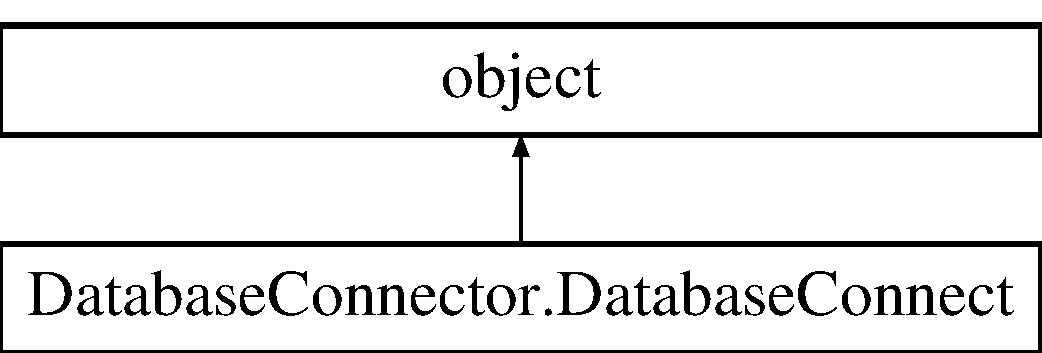
\includegraphics[height=2.000000cm]{classDatabaseConnector_1_1DatabaseConnect}
\end{center}
\end{figure}
\subsection*{Public Member Functions}
\begin{DoxyCompactItemize}
\item 
def \mbox{\hyperlink{classDatabaseConnector_1_1DatabaseConnect_adafc2b78cab3df24b9f1f88990f88ac7}{\+\_\+\+\_\+init\+\_\+\+\_\+}} (self)
\item 
def \mbox{\hyperlink{classDatabaseConnector_1_1DatabaseConnect_a2e58b915bdd35d819f25c110d258adc7}{table\+Exists}} (self, cursor, table\+\_\+name)
\item 
def \mbox{\hyperlink{classDatabaseConnector_1_1DatabaseConnect_a2fea409b9f5b72e8c36f0dd0a8515253}{get\+Next\+Key}} (self, table\+\_\+name)
\begin{DoxyCompactList}\small\item\em Public Functions. \end{DoxyCompactList}\item 
def \mbox{\hyperlink{classDatabaseConnector_1_1DatabaseConnect_a18f9d359811b7bdab423f052fe65e05b}{read\+Table}} (self, table\+\_\+name)
\item 
def \mbox{\hyperlink{classDatabaseConnector_1_1DatabaseConnect_a6e37300433dbbbe0406adb7d969ef2e5}{write\+Data}} (self, table\+\_\+name, new\+\_\+table\+\_\+data)
\item 
def \mbox{\hyperlink{classDatabaseConnector_1_1DatabaseConnect_af67bc1a7983d83e2df140bc3cec92d84}{write\+Device\+Data}} (self, table\+\_\+name, table\+\_\+data)
\item 
def \mbox{\hyperlink{classDatabaseConnector_1_1DatabaseConnect_a9d31fcb5c4b23c692a0488ab8633ba78}{connect}} (self)
\item 
def \mbox{\hyperlink{classDatabaseConnector_1_1DatabaseConnect_aeb9d5d3e55d60d137d938c8ba6f696b7}{disconnect}} (self)
\item 
def \mbox{\hyperlink{classDatabaseConnector_1_1DatabaseConnect_afd3c4da0bc49a45cf43f243bca6fe7f6}{create\+Data\+Table}} (self, table\+\_\+name)
\item 
def \mbox{\hyperlink{classDatabaseConnector_1_1DatabaseConnect_a2ea501b906d72bac48ea7bc92ae87044}{get\+Table\+Names}} (self)
\end{DoxyCompactItemize}
\subsection*{Public Attributes}
\begin{DoxyCompactItemize}
\item 
\mbox{\hyperlink{classDatabaseConnector_1_1DatabaseConnect_a032674c05648a8ba31c2ef9a1363338e}{conn}}
\begin{DoxyCompactList}\small\item\em Variable that determines if connection has been established with database. \end{DoxyCompactList}\item 
\mbox{\hyperlink{classDatabaseConnector_1_1DatabaseConnect_aa3b98ea56e1017172f5cee5e2369e667}{data\+\_\+2ghz\+\_\+query}}
\begin{DoxyCompactList}\small\item\em Variable that is used for tables that contain wifi data on the 2ghz spectrum, query\+: (Key, ts, nou, bits, pkt\+\_\+num, sigs, dr, phyb, phyg, phyn) \end{DoxyCompactList}\end{DoxyCompactItemize}


\subsection{Detailed Description}
\begin{DoxyVerb}Database Object to interact with PostgreSQL database\end{DoxyVerb}
 

\subsection{Constructor \& Destructor Documentation}
\mbox{\Hypertarget{classDatabaseConnector_1_1DatabaseConnect_adafc2b78cab3df24b9f1f88990f88ac7}\label{classDatabaseConnector_1_1DatabaseConnect_adafc2b78cab3df24b9f1f88990f88ac7}} 
\index{Database\+Connector\+::\+Database\+Connect@{Database\+Connector\+::\+Database\+Connect}!\+\_\+\+\_\+init\+\_\+\+\_\+@{\+\_\+\+\_\+init\+\_\+\+\_\+}}
\index{\+\_\+\+\_\+init\+\_\+\+\_\+@{\+\_\+\+\_\+init\+\_\+\+\_\+}!Database\+Connector\+::\+Database\+Connect@{Database\+Connector\+::\+Database\+Connect}}
\subsubsection{\texorpdfstring{\+\_\+\+\_\+init\+\_\+\+\_\+()}{\_\_init\_\_()}}
{\footnotesize\ttfamily def Database\+Connector.\+Database\+Connect.\+\_\+\+\_\+init\+\_\+\+\_\+ (\begin{DoxyParamCaption}\item[{}]{self }\end{DoxyParamCaption})}

\begin{DoxyVerb}Default Constructor for the class\end{DoxyVerb}
 

\subsection{Member Function Documentation}
\mbox{\Hypertarget{classDatabaseConnector_1_1DatabaseConnect_a9d31fcb5c4b23c692a0488ab8633ba78}\label{classDatabaseConnector_1_1DatabaseConnect_a9d31fcb5c4b23c692a0488ab8633ba78}} 
\index{Database\+Connector\+::\+Database\+Connect@{Database\+Connector\+::\+Database\+Connect}!connect@{connect}}
\index{connect@{connect}!Database\+Connector\+::\+Database\+Connect@{Database\+Connector\+::\+Database\+Connect}}
\subsubsection{\texorpdfstring{connect()}{connect()}}
{\footnotesize\ttfamily def Database\+Connector.\+Database\+Connect.\+connect (\begin{DoxyParamCaption}\item[{}]{self }\end{DoxyParamCaption})}

\begin{DoxyVerb}Tries to establish a connection with the database\end{DoxyVerb}
 \mbox{\Hypertarget{classDatabaseConnector_1_1DatabaseConnect_afd3c4da0bc49a45cf43f243bca6fe7f6}\label{classDatabaseConnector_1_1DatabaseConnect_afd3c4da0bc49a45cf43f243bca6fe7f6}} 
\index{Database\+Connector\+::\+Database\+Connect@{Database\+Connector\+::\+Database\+Connect}!create\+Data\+Table@{create\+Data\+Table}}
\index{create\+Data\+Table@{create\+Data\+Table}!Database\+Connector\+::\+Database\+Connect@{Database\+Connector\+::\+Database\+Connect}}
\subsubsection{\texorpdfstring{create\+Data\+Table()}{createDataTable()}}
{\footnotesize\ttfamily def Database\+Connector.\+Database\+Connect.\+create\+Data\+Table (\begin{DoxyParamCaption}\item[{}]{self,  }\item[{}]{table\+\_\+name }\end{DoxyParamCaption})}

\begin{DoxyVerb}Creates table specified by table_name with columns: (Key, ts, nou, bits, pkt_num, sigs, dr, phyb, phyg, phyn). They are all integer values\end{DoxyVerb}
 \mbox{\Hypertarget{classDatabaseConnector_1_1DatabaseConnect_aeb9d5d3e55d60d137d938c8ba6f696b7}\label{classDatabaseConnector_1_1DatabaseConnect_aeb9d5d3e55d60d137d938c8ba6f696b7}} 
\index{Database\+Connector\+::\+Database\+Connect@{Database\+Connector\+::\+Database\+Connect}!disconnect@{disconnect}}
\index{disconnect@{disconnect}!Database\+Connector\+::\+Database\+Connect@{Database\+Connector\+::\+Database\+Connect}}
\subsubsection{\texorpdfstring{disconnect()}{disconnect()}}
{\footnotesize\ttfamily def Database\+Connector.\+Database\+Connect.\+disconnect (\begin{DoxyParamCaption}\item[{}]{self }\end{DoxyParamCaption})}

\begin{DoxyVerb}Disconnects from the database\end{DoxyVerb}
 \mbox{\Hypertarget{classDatabaseConnector_1_1DatabaseConnect_a2fea409b9f5b72e8c36f0dd0a8515253}\label{classDatabaseConnector_1_1DatabaseConnect_a2fea409b9f5b72e8c36f0dd0a8515253}} 
\index{Database\+Connector\+::\+Database\+Connect@{Database\+Connector\+::\+Database\+Connect}!get\+Next\+Key@{get\+Next\+Key}}
\index{get\+Next\+Key@{get\+Next\+Key}!Database\+Connector\+::\+Database\+Connect@{Database\+Connector\+::\+Database\+Connect}}
\subsubsection{\texorpdfstring{get\+Next\+Key()}{getNextKey()}}
{\footnotesize\ttfamily def Database\+Connector.\+Database\+Connect.\+get\+Next\+Key (\begin{DoxyParamCaption}\item[{}]{self,  }\item[{}]{table\+\_\+name }\end{DoxyParamCaption})}



Public Functions. 

\begin{DoxyVerb}Gets the next key needed to upload to the database, insures that there are no key conflicts\end{DoxyVerb}
 \mbox{\Hypertarget{classDatabaseConnector_1_1DatabaseConnect_a2ea501b906d72bac48ea7bc92ae87044}\label{classDatabaseConnector_1_1DatabaseConnect_a2ea501b906d72bac48ea7bc92ae87044}} 
\index{Database\+Connector\+::\+Database\+Connect@{Database\+Connector\+::\+Database\+Connect}!get\+Table\+Names@{get\+Table\+Names}}
\index{get\+Table\+Names@{get\+Table\+Names}!Database\+Connector\+::\+Database\+Connect@{Database\+Connector\+::\+Database\+Connect}}
\subsubsection{\texorpdfstring{get\+Table\+Names()}{getTableNames()}}
{\footnotesize\ttfamily def Database\+Connector.\+Database\+Connect.\+get\+Table\+Names (\begin{DoxyParamCaption}\item[{}]{self }\end{DoxyParamCaption})}

\begin{DoxyVerb}Returns a list of table names in the database\end{DoxyVerb}
 \mbox{\Hypertarget{classDatabaseConnector_1_1DatabaseConnect_a18f9d359811b7bdab423f052fe65e05b}\label{classDatabaseConnector_1_1DatabaseConnect_a18f9d359811b7bdab423f052fe65e05b}} 
\index{Database\+Connector\+::\+Database\+Connect@{Database\+Connector\+::\+Database\+Connect}!read\+Table@{read\+Table}}
\index{read\+Table@{read\+Table}!Database\+Connector\+::\+Database\+Connect@{Database\+Connector\+::\+Database\+Connect}}
\subsubsection{\texorpdfstring{read\+Table()}{readTable()}}
{\footnotesize\ttfamily def Database\+Connector.\+Database\+Connect.\+read\+Table (\begin{DoxyParamCaption}\item[{}]{self,  }\item[{}]{table\+\_\+name }\end{DoxyParamCaption})}

\begin{DoxyVerb}Returns the entire content of table_name\end{DoxyVerb}
 \mbox{\Hypertarget{classDatabaseConnector_1_1DatabaseConnect_a2e58b915bdd35d819f25c110d258adc7}\label{classDatabaseConnector_1_1DatabaseConnect_a2e58b915bdd35d819f25c110d258adc7}} 
\index{Database\+Connector\+::\+Database\+Connect@{Database\+Connector\+::\+Database\+Connect}!table\+Exists@{table\+Exists}}
\index{table\+Exists@{table\+Exists}!Database\+Connector\+::\+Database\+Connect@{Database\+Connector\+::\+Database\+Connect}}
\subsubsection{\texorpdfstring{table\+Exists()}{tableExists()}}
{\footnotesize\ttfamily def Database\+Connector.\+Database\+Connect.\+table\+Exists (\begin{DoxyParamCaption}\item[{}]{self,  }\item[{}]{cursor,  }\item[{}]{table\+\_\+name }\end{DoxyParamCaption})}

\begin{DoxyVerb}Checks if table exists in database\end{DoxyVerb}
 \mbox{\Hypertarget{classDatabaseConnector_1_1DatabaseConnect_a6e37300433dbbbe0406adb7d969ef2e5}\label{classDatabaseConnector_1_1DatabaseConnect_a6e37300433dbbbe0406adb7d969ef2e5}} 
\index{Database\+Connector\+::\+Database\+Connect@{Database\+Connector\+::\+Database\+Connect}!write\+Data@{write\+Data}}
\index{write\+Data@{write\+Data}!Database\+Connector\+::\+Database\+Connect@{Database\+Connector\+::\+Database\+Connect}}
\subsubsection{\texorpdfstring{write\+Data()}{writeData()}}
{\footnotesize\ttfamily def Database\+Connector.\+Database\+Connect.\+write\+Data (\begin{DoxyParamCaption}\item[{}]{self,  }\item[{}]{table\+\_\+name,  }\item[{}]{new\+\_\+table\+\_\+data }\end{DoxyParamCaption})}

\begin{DoxyVerb}Writes data to table of PostgreSQL database, input must be in this from: Key, ts, nou, bits, pkt_num, sigs, dr, phyb, phyg, phyn. Where all values are integers\end{DoxyVerb}
 \mbox{\Hypertarget{classDatabaseConnector_1_1DatabaseConnect_af67bc1a7983d83e2df140bc3cec92d84}\label{classDatabaseConnector_1_1DatabaseConnect_af67bc1a7983d83e2df140bc3cec92d84}} 
\index{Database\+Connector\+::\+Database\+Connect@{Database\+Connector\+::\+Database\+Connect}!write\+Device\+Data@{write\+Device\+Data}}
\index{write\+Device\+Data@{write\+Device\+Data}!Database\+Connector\+::\+Database\+Connect@{Database\+Connector\+::\+Database\+Connect}}
\subsubsection{\texorpdfstring{write\+Device\+Data()}{writeDeviceData()}}
{\footnotesize\ttfamily def Database\+Connector.\+Database\+Connect.\+write\+Device\+Data (\begin{DoxyParamCaption}\item[{}]{self,  }\item[{}]{table\+\_\+name,  }\item[{}]{table\+\_\+data }\end{DoxyParamCaption})}

\begin{DoxyVerb}This function takes a list of [key, mac addr, ip addr] specified by table_data and adds it to database specified by table_name\end{DoxyVerb}
 

\subsection{Member Data Documentation}
\mbox{\Hypertarget{classDatabaseConnector_1_1DatabaseConnect_a032674c05648a8ba31c2ef9a1363338e}\label{classDatabaseConnector_1_1DatabaseConnect_a032674c05648a8ba31c2ef9a1363338e}} 
\index{Database\+Connector\+::\+Database\+Connect@{Database\+Connector\+::\+Database\+Connect}!conn@{conn}}
\index{conn@{conn}!Database\+Connector\+::\+Database\+Connect@{Database\+Connector\+::\+Database\+Connect}}
\subsubsection{\texorpdfstring{conn}{conn}}
{\footnotesize\ttfamily Database\+Connect.\+conn}



Variable that determines if connection has been established with database. 

\mbox{\Hypertarget{classDatabaseConnector_1_1DatabaseConnect_aa3b98ea56e1017172f5cee5e2369e667}\label{classDatabaseConnector_1_1DatabaseConnect_aa3b98ea56e1017172f5cee5e2369e667}} 
\index{Database\+Connector\+::\+Database\+Connect@{Database\+Connector\+::\+Database\+Connect}!data\+\_\+2ghz\+\_\+query@{data\+\_\+2ghz\+\_\+query}}
\index{data\+\_\+2ghz\+\_\+query@{data\+\_\+2ghz\+\_\+query}!Database\+Connector\+::\+Database\+Connect@{Database\+Connector\+::\+Database\+Connect}}
\subsubsection{\texorpdfstring{data\+\_\+2ghz\+\_\+query}{data\_2ghz\_query}}
{\footnotesize\ttfamily Database\+Connect.\+data\+\_\+2ghz\+\_\+query}



Variable that is used for tables that contain wifi data on the 2ghz spectrum, query\+: (Key, ts, nou, bits, pkt\+\_\+num, sigs, dr, phyb, phyg, phyn) 



The documentation for this class was generated from the following file\+:\begin{DoxyCompactItemize}
\item 
\mbox{\hyperlink{DatabaseConnector_8py}{Database\+Connector.\+py}}\end{DoxyCompactItemize}

\chapter{File Documentation}
\hypertarget{DatabaseConnect_8cpp}{}\section{Database\+Connect.\+cpp File Reference}
\label{DatabaseConnect_8cpp}\index{Database\+Connect.\+cpp@{Database\+Connect.\+cpp}}
{\ttfamily \#include \char`\"{}Database\+Connect.\+hpp\char`\"{}}\newline
{\ttfamily \#include $<$string$>$}\newline
{\ttfamily \#include $<$vector$>$}\newline

\hypertarget{DatabaseConnect_8hpp}{}\section{Database\+Connect.\+hpp File Reference}
\label{DatabaseConnect_8hpp}\index{Database\+Connect.\+hpp@{Database\+Connect.\+hpp}}
{\ttfamily \#include $<$stdio.\+h$>$}\newline
{\ttfamily \#include $<$string$>$}\newline
{\ttfamily \#include $<$stdlib.\+h$>$}\newline
{\ttfamily \#include $<$iostream$>$}\newline
{\ttfamily \#include $<$vector$>$}\newline
{\ttfamily \#include $<$postgresql/libpq-\/fe.\+h$>$}\newline
\subsection*{Classes}
\begin{DoxyCompactItemize}
\item 
class \mbox{\hyperlink{classDatabaseConnect}{Database\+Connect}}
\begin{DoxyCompactList}\small\item\em Class with functions for \mbox{\hyperlink{classDatabaseConnect}{Database\+Connect}} and \mbox{\hyperlink{parser5_8cpp}{parser5.\+cpp}}. \end{DoxyCompactList}\end{DoxyCompactItemize}

\hypertarget{DatabaseConnector_8py}{}\section{Database\+Connector.\+py File Reference}
\label{DatabaseConnector_8py}\index{Database\+Connector.\+py@{Database\+Connector.\+py}}
\subsection*{Classes}
\begin{DoxyCompactItemize}
\item 
class \mbox{\hyperlink{classDatabaseConnector_1_1DatabaseConnect}{Database\+Connector.\+Database\+Connect}}
\end{DoxyCompactItemize}
\subsection*{Namespaces}
\begin{DoxyCompactItemize}
\item 
 \mbox{\hyperlink{namespaceDatabaseConnector}{Database\+Connector}}
\end{DoxyCompactItemize}

\hypertarget{device__emitter_8py}{}\section{device\+\_\+emitter.\+py File Reference}
\label{device__emitter_8py}\index{device\+\_\+emitter.\+py@{device\+\_\+emitter.\+py}}
\subsection*{Namespaces}
\begin{DoxyCompactItemize}
\item 
 \mbox{\hyperlink{namespacedevice__emitter}{device\+\_\+emitter}}
\end{DoxyCompactItemize}
\subsection*{Functions}
\begin{DoxyCompactItemize}
\item 
def \mbox{\hyperlink{namespacedevice__emitter_a37babfaa6ea3bbb358c94516521f9442}{device\+\_\+emitter.\+txt\+\_\+reader}} (input\+\_\+file)
\item 
def \mbox{\hyperlink{namespacedevice__emitter_a3d36fb9ab99c12fae8dff6cae0b9c309}{device\+\_\+emitter.\+data\+\_\+upload}} (table\+\_\+name, input\+\_\+ip, input\+\_\+mac)
\end{DoxyCompactItemize}
\subsection*{Variables}
\begin{DoxyCompactItemize}
\item 
string \mbox{\hyperlink{namespacedevice__emitter_ae71d803969e8f98677e12dc98159d6de}{device\+\_\+emitter.\+table\+\_\+name}} = \char`\"{}ip\char`\"{}
\item 
\mbox{\hyperlink{namespacedevice__emitter_a0559bc31b21eed1581ff97fccbbd75d7}{device\+\_\+emitter.\+db}} = dc.\+Database\+Connect()
\item 
\mbox{\hyperlink{namespacedevice__emitter_a41adb72e6db041039a6416f891820c45}{device\+\_\+emitter.\+table\+\_\+contents}} = db.\+read\+Table(table\+\_\+name)
\item 
dictionary \mbox{\hyperlink{namespacedevice__emitter_a803e1fc15d8f8f4445053a2b36e7ac0b}{device\+\_\+emitter.\+pi\+\_\+details}} = \{\}
\item 
string \mbox{\hyperlink{namespacedevice__emitter_adffb57ad574487e214cf5a3033abbae8}{device\+\_\+emitter.\+ip\+\_\+txt}} = \char`\"{}ip.\+txt\char`\"{}
\item 
def \mbox{\hyperlink{namespacedevice__emitter_accb17d54f29bb0b5cc59b7f81d3ed0f3}{device\+\_\+emitter.\+ip\+\_\+addr}} = txt\+\_\+reader(ip\+\_\+txt)
\item 
string \mbox{\hyperlink{namespacedevice__emitter_ad664a79343b74123be899bb0752a6fb1}{device\+\_\+emitter.\+mac\+\_\+txt}} = \char`\"{}mac.\+txt\char`\"{}
\item 
def \mbox{\hyperlink{namespacedevice__emitter_ac0f4af4fd7abf558f1b2ad320894f040}{device\+\_\+emitter.\+mac\+\_\+addr}} = txt\+\_\+reader(mac\+\_\+txt)
\item 
dictionary \mbox{\hyperlink{namespacedevice__emitter_ae3817f26c179f6e6e62775fcabaa1bc9}{device\+\_\+emitter.\+database\+\_\+ip}} = pi\+\_\+details\mbox{[}pi\+\_\+iterator+1\mbox{]}\mbox{[}1\mbox{]}
\item 
int \mbox{\hyperlink{namespacedevice__emitter_a1797fb3f5a71e4f2212c4a43454141a2}{device\+\_\+emitter.\+ip\+\_\+check}} = 0
\item 
int \mbox{\hyperlink{namespacedevice__emitter_ae5bc45db5e138407237ffd7c0d38afba}{device\+\_\+emitter.\+mac\+\_\+check}} = 0
\item 
dictionary \mbox{\hyperlink{namespacedevice__emitter_a74cf5779300d3c95c075f304d1340771}{device\+\_\+emitter.\+database\+\_\+mac}} = pi\+\_\+details\mbox{[}pi\+\_\+iterator+1\mbox{]}\mbox{[}0\mbox{]}
\end{DoxyCompactItemize}

\hypertarget{device__reader_8py}{}\section{device\+\_\+reader.\+py File Reference}
\label{device__reader_8py}\index{device\+\_\+reader.\+py@{device\+\_\+reader.\+py}}
\subsection*{Namespaces}
\begin{DoxyCompactItemize}
\item 
 \mbox{\hyperlink{namespacedevice__reader}{device\+\_\+reader}}
\end{DoxyCompactItemize}
\subsection*{Variables}
\begin{DoxyCompactItemize}
\item 
string \mbox{\hyperlink{namespacedevice__reader_aad8c1a079cd59349e6fe8da74a150b4c}{device\+\_\+reader.\+table\+\_\+name}} = \char`\"{}ip\char`\"{}
\item 
\mbox{\hyperlink{namespacedevice__reader_aef8ef243dde3f69875aa5ff4b68a35c9}{device\+\_\+reader.\+db}} = dc.\+Database\+Connect()
\item 
\mbox{\hyperlink{namespacedevice__reader_a5ee29ddcc8e6bbf93f8557da0f4a9853}{device\+\_\+reader.\+table\+\_\+contents}} = db.\+read\+Table(table\+\_\+name)
\item 
dictionary \mbox{\hyperlink{namespacedevice__reader_a05ed01d1cd5e9a1a511ee479e231f81c}{device\+\_\+reader.\+device\+\_\+details}} = \{\}
\item 
\mbox{\hyperlink{namespacedevice__reader_ad7cd4038fd9f67b2a6718b9bfb195a62}{device\+\_\+reader.\+key}}
\end{DoxyCompactItemize}

\hypertarget{parser5_8cpp}{}\section{parser5.\+cpp File Reference}
\label{parser5_8cpp}\index{parser5.\+cpp@{parser5.\+cpp}}
{\ttfamily \#include $<$iostream$>$}\newline
{\ttfamily \#include $<$tins/tins.\+h$>$}\newline
{\ttfamily \#include $<$bitset$>$}\newline
{\ttfamily \#include $<$stddef.\+h$>$}\newline
{\ttfamily \#include $<$string$>$}\newline
{\ttfamily \#include $<$vector$>$}\newline
{\ttfamily \#include $<$boost/filesystem.\+hpp$>$}\newline
{\ttfamily \#include \char`\"{}Database\+Connect.\+hpp\char`\"{}}\newline
{\ttfamily \#include $<$algorithm$>$}\newline
\subsection*{Functions}
\begin{DoxyCompactItemize}
\item 
int \mbox{\hyperlink{parser5_8cpp_a0ddf1224851353fc92bfbff6f499fa97}{main}} (int argc, char $\ast$argv\mbox{[}$\,$\mbox{]})
\end{DoxyCompactItemize}


\subsection{Detailed Description}
\begin{DoxyAuthor}{Author}
Francisco Viramontes
\end{DoxyAuthor}
Description\+: This is a pcap parser that reads pcap files from a specified directory (specified by std\+::string path) and reads statistics like number of users, bits sent over the network, and fits them into a vector that represents the statistical analysis for that second.

Input\+: At least one pcap file in the folder specified in std\+::string path. T\+HE P\+C\+AP F\+I\+LE M\+U\+ST BE S\+N\+I\+F\+F\+ED V\+IA W\+I\+R\+E\+L\+E\+SS N\+OT E\+T\+H\+E\+R\+N\+E\+T! T\+HE P\+R\+O\+G\+R\+AM W\+I\+LL N\+OT W\+O\+R\+K!

Output\+: A few statements printed on terminal, specifying the status of the interaction with the Postgre\+S\+QL database. Uploads a row of sql data to the Postgre\+S\+QL database. Details of the row follow as such\+: Timestamp, Number of Users, Total Bits, Total Packets, Avg Signal Strength, Avg Data Rate, 802.\+11a Bits, 802.\+11n bits

TO C\+O\+M\+P\+I\+LE\+: g++ \mbox{\hyperlink{parser5_8cpp}{parser5.\+cpp}} \mbox{\hyperlink{DatabaseConnect_8cpp}{Database\+Connect.\+cpp}} -\/ltins -\/lboost\+\_\+system -\/lboost\+\_\+filesystem -\/lpq -\/o {\itshape executable\+\_\+name} TO C\+A\+P\+T\+U\+RE D\+A\+TA\+: tshark -\/i {\itshape Wi\+Fi Interface} -\/I -\/a duration\+:60 -\/b duration\+:1 -\/w data.\+pcap {\itshape !}!$\ast$!$\ast$!$\ast$!$\ast$!$\ast$\+M\+A\+KE S\+U\+RE Y\+O\+UR W\+I\+R\+E\+L\+E\+SS I\+N\+T\+E\+R\+F\+A\+CE IS IN M\+O\+N\+I\+T\+OR M\+O\+D\+E$\ast$!$\ast$!$\ast$!$\ast$!$\ast$!$\ast$!$\ast$!$\ast$! 

\subsection{Function Documentation}
\mbox{\Hypertarget{parser5_8cpp_a0ddf1224851353fc92bfbff6f499fa97}\label{parser5_8cpp_a0ddf1224851353fc92bfbff6f499fa97}} 
\index{parser5.\+cpp@{parser5.\+cpp}!main@{main}}
\index{main@{main}!parser5.\+cpp@{parser5.\+cpp}}
\subsubsection{\texorpdfstring{main()}{main()}}
{\footnotesize\ttfamily int main (\begin{DoxyParamCaption}\item[{int}]{argc,  }\item[{char $\ast$}]{argv\mbox{[}$\,$\mbox{]} }\end{DoxyParamCaption})}

This is a pcap parser that reads pcap files from a specified directory (specified by std\+::string path) and reads statistics like number of users, bits sent over the network, and fits them into a std\+::vector array that represents the statistical analysis for that second.

Declaring table name to write to

Creates a local cache of recent files parsed so that we don\textquotesingle{}t re-\/parse a pcap file

The string path is to go to the selected path to parse pcap files 
\hypertarget{README_8md}{}\section{R\+E\+A\+D\+M\+E.\+md File Reference}
\label{README_8md}\index{R\+E\+A\+D\+M\+E.\+md@{R\+E\+A\+D\+M\+E.\+md}}

\hypertarget{time__series2_8py}{}\section{time\+\_\+series2.\+py File Reference}
\label{time__series2_8py}\index{time\+\_\+series2.\+py@{time\+\_\+series2.\+py}}
\subsection*{Namespaces}
\begin{DoxyCompactItemize}
\item 
 \mbox{\hyperlink{namespacetime__series2}{time\+\_\+series2}}
\end{DoxyCompactItemize}
\subsection*{Functions}
\begin{DoxyCompactItemize}
\item 
def \mbox{\hyperlink{namespacetime__series2_a91a50d414e62104b3c4df302683fa374}{time\+\_\+series2.\+mean}} (values)
\item 
def \mbox{\hyperlink{namespacetime__series2_a2fb326ca63610119cde08d76b52599fe}{time\+\_\+series2.\+sample\+\_\+var}} (values, sample\+\_\+mean=None)
\item 
def \mbox{\hyperlink{namespacetime__series2_afb06c28c1769268d33ce21dfae5d064a}{time\+\_\+series2.\+covariance}} (x, mean\+\_\+x, y, mean\+\_\+y)
\item 
def \mbox{\hyperlink{namespacetime__series2_ab7308a3396727b46466322d617ea0af5}{time\+\_\+series2.\+sub\+\_\+sample}} (sample\+\_\+arr, sample\+\_\+size)
\item 
def \mbox{\hyperlink{namespacetime__series2_a831b2ebbb3b93f1a189a11b798867bf2}{time\+\_\+series2.\+avg\+\_\+sample}} (sample\+\_\+arr, sample\+\_\+size)
\item 
def \mbox{\hyperlink{namespacetime__series2_a31fa5faf99bfb7d4e08f53e5f04d77e0}{time\+\_\+series2.\+grab\+\_\+n}} (array, n)
\item 
def \mbox{\hyperlink{namespacetime__series2_a82eef0f2d8234468ad48ed485a433494}{time\+\_\+series2.\+grab\+\_\+nz}} (array, n, z)
\item 
def \mbox{\hyperlink{namespacetime__series2_a132464d53987913f012c331095a66ccd}{time\+\_\+series2.\+G\+P\+\_\+prep}} (train, test, avg\+\_\+samp, sub\+\_\+samp\+\_\+begin, sub\+\_\+samp\+\_\+end, window)
\end{DoxyCompactItemize}
\subsection*{Variables}
\begin{DoxyCompactItemize}
\item 
\mbox{\hyperlink{namespacetime__series2_a4ad96ae33e961d2a7b9254dcf7705ab1}{time\+\_\+series2.\+threshold}}
\item 
list \mbox{\hyperlink{namespacetime__series2_ac28cc09905078b265b7b43c5a572bc15}{time\+\_\+series2.\+timestamps}} = \mbox{[}$\,$\mbox{]}
\item 
list \mbox{\hyperlink{namespacetime__series2_a97c4b20f0435fa06589a14b07d581ba4}{time\+\_\+series2.\+nou}} = \mbox{[}$\,$\mbox{]}
\item 
list \mbox{\hyperlink{namespacetime__series2_a482617ebda72aedc92277cb1705e039e}{time\+\_\+series2.\+nou\+\_\+tst}} = \mbox{[}$\,$\mbox{]}
\item 
list \mbox{\hyperlink{namespacetime__series2_af73dec23edfc91f6252482247ec3e77a}{time\+\_\+series2.\+bits}} = \mbox{[}$\,$\mbox{]}
\item 
list \mbox{\hyperlink{namespacetime__series2_a2756c0f213fa5f5d2b6cb8fec406006f}{time\+\_\+series2.\+bits\+\_\+tst}} = \mbox{[}$\,$\mbox{]}
\item 
list \mbox{\hyperlink{namespacetime__series2_ab18c2a5668ac375ae8024899566ec9cb}{time\+\_\+series2.\+pkt\+Num}} = \mbox{[}$\,$\mbox{]}
\item 
list \mbox{\hyperlink{namespacetime__series2_a82cbfdb5aaf630b9b2b8a795f8ec71a4}{time\+\_\+series2.\+pkt\+\_\+tst}} = \mbox{[}$\,$\mbox{]}
\item 
list \mbox{\hyperlink{namespacetime__series2_a7f4c741d69814ab642aaeb0d3ba3c6dd}{time\+\_\+series2.\+sigS}} = \mbox{[}$\,$\mbox{]}
\item 
list \mbox{\hyperlink{namespacetime__series2_afe062e2326a14ed5b7bb7084a7ec5be3}{time\+\_\+series2.\+sig\+S\+\_\+tst}} = \mbox{[}$\,$\mbox{]}
\item 
list \mbox{\hyperlink{namespacetime__series2_add60d2a933f0e3175a7c67f66e4aca2d}{time\+\_\+series2.\+data\+Rate}} = \mbox{[}$\,$\mbox{]}
\item 
list \mbox{\hyperlink{namespacetime__series2_a07fb1c09cd6557a4f473012b13676236}{time\+\_\+series2.\+d\+R\+\_\+tst}} = \mbox{[}$\,$\mbox{]}
\item 
list \mbox{\hyperlink{namespacetime__series2_a02d0468d51f7289b53b70785a2297001}{time\+\_\+series2.\+phyB}} = \mbox{[}$\,$\mbox{]}
\item 
list \mbox{\hyperlink{namespacetime__series2_a57a31949fdcc87477da71be37f2a843f}{time\+\_\+series2.\+b\+\_\+tst}} = \mbox{[}$\,$\mbox{]}
\item 
list \mbox{\hyperlink{namespacetime__series2_a33d26c4c9e21812d76047ef5d806a909}{time\+\_\+series2.\+phyG}} = \mbox{[}$\,$\mbox{]}
\item 
list \mbox{\hyperlink{namespacetime__series2_a8ae6164c022bbafc01611a6801bc0f61}{time\+\_\+series2.\+g\+\_\+tst}} = \mbox{[}$\,$\mbox{]}
\item 
list \mbox{\hyperlink{namespacetime__series2_adcb42f8de34d804df871439dac54f26d}{time\+\_\+series2.\+phyN}} = \mbox{[}$\,$\mbox{]}
\item 
list \mbox{\hyperlink{namespacetime__series2_a6473b442b1cc4cbcfee1f06b95739529}{time\+\_\+series2.\+n\+\_\+tst}} = \mbox{[}$\,$\mbox{]}
\item 
\mbox{\hyperlink{namespacetime__series2_aa3dc64ee4f5d2e030faa61cfe845a994}{time\+\_\+series2.\+db}} = dc.\+Database\+Connect()
\item 
string \mbox{\hyperlink{namespacetime__series2_a34db5677db4e9381ee013b03a4e01231}{time\+\_\+series2.\+train\+\_\+table}} = \char`\"{}pi\+\_\+mon\char`\"{}
\item 
string \mbox{\hyperlink{namespacetime__series2_aae4b3d023bcc07d4610b83f328c9c817}{time\+\_\+series2.\+test\+\_\+table}} = \char`\"{}pi\+\_\+sun\char`\"{}
\item 
\mbox{\hyperlink{namespacetime__series2_a217725c41e0be8eff877ccf0738ca225}{time\+\_\+series2.\+train}} = db.\+read\+Table(train\+\_\+table)
\item 
\mbox{\hyperlink{namespacetime__series2_a1db23c9847b01280de0f7b35c02ec33d}{time\+\_\+series2.\+test}} = db.\+read\+Table(test\+\_\+table)
\item 
\mbox{\hyperlink{namespacetime__series2_a5eb1f8d582696414c5a074d2bdaeb4f5}{time\+\_\+series2.\+key}}
\item 
list \mbox{\hyperlink{namespacetime__series2_a19f3e3f5bd2694a9a461163b260e68a4}{time\+\_\+series2.\+training\+\_\+data}}
\item 
list \mbox{\hyperlink{namespacetime__series2_ac919557d9139430fa99c37bb9847b34a}{time\+\_\+series2.\+test\+\_\+data}}
\item 
list \mbox{\hyperlink{namespacetime__series2_aca78083d23e0850ea4120fa6817af6fb}{time\+\_\+series2.\+labels}}
\item 
def \mbox{\hyperlink{namespacetime__series2_a2675eebe825f166195eff20a30027b0b}{time\+\_\+series2.\+short\+\_\+nou}} = avg\+\_\+sample(nou, 1800)
\item 
def \mbox{\hyperlink{namespacetime__series2_a1f91a36b8475489b7a12b6ade0010039}{time\+\_\+series2.\+short\+\_\+bits}} = avg\+\_\+sample(bits, 1800)
\item 
def \mbox{\hyperlink{namespacetime__series2_ab12db667114a1ed12973125874bc16d4}{time\+\_\+series2.\+short\+\_\+pkt\+Num}} = avg\+\_\+sample(pkt\+Num, 1800)
\item 
def \mbox{\hyperlink{namespacetime__series2_a606a9c83f25e85d3f3433dc36a593350}{time\+\_\+series2.\+short\+\_\+sigS}} = avg\+\_\+sample(sigS, 1800)
\item 
def \mbox{\hyperlink{namespacetime__series2_a0ca06fc00c13efdb759ffc0a7773bee5}{time\+\_\+series2.\+short\+\_\+dR}} = avg\+\_\+sample(data\+Rate, 1800)
\item 
int \mbox{\hyperlink{namespacetime__series2_a090c1e69b2375fcbd478928c1e306abf}{time\+\_\+series2.\+sample\+\_\+start}} = 0
\item 
int \mbox{\hyperlink{namespacetime__series2_ad170197f80cacfa1a597f0cc81af1ed5}{time\+\_\+series2.\+sample\+\_\+end}} = 100
\item 
int \mbox{\hyperlink{namespacetime__series2_abbcc8a8aa4c18c3850b74368b2728790}{time\+\_\+series2.\+sample\+\_\+window}} = 15
\item 
\mbox{\hyperlink{namespacetime__series2_aa8462353b2fa60dd1b67e2d81b1f53a5}{time\+\_\+series2.\+kernel1}} = LK(sigma\+\_\+0 = 1, sigma\+\_\+0\+\_\+bounds = (1e-\/1, 1e1))
\item 
\mbox{\hyperlink{namespacetime__series2_acf4bc51affffd98b22fcd3442438fff0}{time\+\_\+series2.\+kernel2}} = CK(constant\+\_\+value=1)
\item 
\mbox{\hyperlink{namespacetime__series2_afa3d3c8fdd4d9a88bf7e9e05b4bb806d}{time\+\_\+series2.\+kernel3}} = WK(0.\+1)
\item 
\mbox{\hyperlink{namespacetime__series2_a79d2d803d9f27eb4ed08932199d79a23}{time\+\_\+series2.\+kernel}} = Sum(kernel1, kernel2)
\item 
\mbox{\hyperlink{namespacetime__series2_abd0932f2ea87fc90f945a626050ecc14}{time\+\_\+series2.\+gp}}
\item 
\mbox{\hyperlink{namespacetime__series2_af8e48fc6d3d4ad2c551a1b3df864aa51}{time\+\_\+series2.\+total\+\_\+samp}}
\item 
\mbox{\hyperlink{namespacetime__series2_a9ad02e52f2e578dff25a50245476fb4d}{time\+\_\+series2.\+Xtr}}
\item 
\mbox{\hyperlink{namespacetime__series2_a048fc1f5052ecd0ac42a809d13599ff0}{time\+\_\+series2.\+Ytr}}
\item 
\mbox{\hyperlink{namespacetime__series2_aff22e5d05c2a50ecb36a4f87019d31fb}{time\+\_\+series2.\+Xtst}}
\item 
\mbox{\hyperlink{namespacetime__series2_af29c132f3c4ad21f3ce71ca94bd5e811}{time\+\_\+series2.\+Ycomp}}
\item 
\mbox{\hyperlink{namespacetime__series2_ad545baebbafca44d770c7184debd3ebb}{time\+\_\+series2.\+Ytst}}
\item 
list \mbox{\hyperlink{namespacetime__series2_a22428a1c2732c1fe95c8f9bc060b1a56}{time\+\_\+series2.\+Xtr\+\_\+1}} = \mbox{[}Xtr\mbox{[}i\mbox{]} for i in range(sample\+\_\+window, sample\+\_\+end)\mbox{]}
\item 
\mbox{\hyperlink{namespacetime__series2_adc3835a1aee5e6024fcf327d2fac0f08}{time\+\_\+series2.\+y\+\_\+pred}}
\item 
\mbox{\hyperlink{namespacetime__series2_a41dcf5a15bbf43705317edb2c4917073}{time\+\_\+series2.\+y\+\_\+sigma}}
\item 
\mbox{\hyperlink{namespacetime__series2_a6438463f77ead66c93e77557813fc843}{time\+\_\+series2.\+return\+\_\+std}}
\item 
list \mbox{\hyperlink{namespacetime__series2_a8bc1ba75be8714303adfe853be1fdfa7}{time\+\_\+series2.\+result\+\_\+time}} = \mbox{[}g+1 for g in range(sample\+\_\+window, sample\+\_\+end)\mbox{]}
\item 
string \mbox{\hyperlink{namespacetime__series2_a1cde44ae6d15f2025f459a56910bb627}{time\+\_\+series2.\+s}} = \char`\"{}training interval between \char`\"{}+str(result\+\_\+time\mbox{[}0\mbox{]})+\char`\"{} and \char`\"{}+str(result\+\_\+time\mbox{[}-\/1\mbox{]})+\textbackslash{}
\item 
list \mbox{\hyperlink{namespacetime__series2_aede1d0cfe7385a32db06215b98af807c}{time\+\_\+series2.\+ylab}} = labels\mbox{[}z\mbox{]}
\item 
\mbox{\hyperlink{namespacetime__series2_adf5da4818165639941e8e5fbd59b8079}{time\+\_\+series2.\+label}}
\item 
string \mbox{\hyperlink{namespacetime__series2_ab96e591ad1ad71d491e9c0911dbcfb3f}{time\+\_\+series2.\+G\+P\+\_\+xlabel}} = \char`\"{}time interval between \char`\"{}+str(result\+\_\+time\mbox{[}0\mbox{]})+\char`\"{} and \char`\"{}+str(result\+\_\+time\mbox{[}-\/1\mbox{]})+\textbackslash{}
\item 
list \mbox{\hyperlink{namespacetime__series2_a21760fd1a155e704a4ebc53bcdd542dd}{time\+\_\+series2.\+G\+P\+\_\+ylabel}} = labels\mbox{[}z\mbox{]}
\item 
string \mbox{\hyperlink{namespacetime__series2_abbce76511798b545cbd2d31ff635e1e0}{time\+\_\+series2.\+G\+P\+\_\+dataplot\+\_\+title}} = \char`\"{}Using \char`\"{}+str(gp.\+get\+\_\+params()\mbox{[}\textquotesingle{}kernel\textquotesingle{}\mbox{]})+\char`\"{} kernel\textbackslash{}nwith \char`\"{}+str(total\+\_\+samp)+\char`\"{} averaged training samples\textbackslash{}nand \char`\"{}+str(sample\+\_\+end)+\textbackslash{}
\item 
\mbox{\hyperlink{namespacetime__series2_ab77f3dac8f9c1b3b736d630b63ea8d35}{time\+\_\+series2.\+alpha}}
\item 
\mbox{\hyperlink{namespacetime__series2_ab333f29befe468b5e60f2cfee44c97d2}{time\+\_\+series2.\+fc}}
\item 
\mbox{\hyperlink{namespacetime__series2_a99eb3f92724746be5d1ddd4434cb4b4f}{time\+\_\+series2.\+ec}}
\end{DoxyCompactItemize}

%--- End generated contents ---

% Index
\backmatter
\newpage
\phantomsection
\clearemptydoublepage
\addcontentsline{toc}{chapter}{\indexname}
\printindex

\end{document}
